%
% The standard LaTeX article class is close to what is needed for an MPhys project report
\documentclass[12pt]{article}

% The following package makes the necessary tweaks to comply with the formatting requirements.
% It also provides a standardised title page, and will warn you if the main text is too long.
\usepackage{mphysproject}
%
%% DO NOT GO CHANGING THE FONT SIZE OR MARGINS! If your main text doesn't fit within 50 pages,
%% you will have to cut stuff out.
%
%% REMEMBER: The target length is around 35 pages
%

% The formatting of the document can be enhanced by loading extra packages.
%
% An essential package is `graphicx', which is loaded by the mphysproject package so you don't
% need to load this yourself. This allows you to include figures using the \includegraphics command.
% To get more information about a package, type texdoc <package> on the Unix command line,
% substituting <package> with the name of the package, e.g., texdoc graphicx
%
% For a wider variety of mathematical environments, symbols and formatting options:
%\usepackage{amsmath,amssymb}
%
% If you want to use colour in the text
%\usepackage{color}
%
% If you want to put figures side by side with separate captions
%\usepackage{subfigure}
% For sub figures, subfigure package is depreciated.
\usepackage{subcaption}
% If you happen to dislike the standard TeX fonts
%\usepackage{times}
%
% If you include any URLs in your text and/or want to make cross-references clickable, include one of the following
% two lines
\usepackage{hyperref}  % This enables hyperlinks but leaves them in black, which is best for printing
%\usepackage[colorlinks=true]{hyperref} % This colours the hyperlinks, which is better for screen reading
% For Bra-Ket notation.
\usepackage{braket}
% For pictures.
\usepackage{tikz}
% For creating data plots.
\usepackage{pgfplots}
% For maths symbols.
\usepackage{amsfonts}
% For colon equals.
\usepackage{mathtools}
% For adding todo notes.
\usepackage[textsize=tiny]{todonotes}
% For nice bold vector symbols.
\usepackage{bm}
% For nicer fractions.
\usepackage[nice]{nicefrac}
% For Tiny font size.
\usepackage{lmodern}
% For more floats
\usepackage{morefloats}

\begin{document}

\title{Accelerated Tempering Dynamics in HMC Simulations of Lattice Field Theory} % Place your project title in here
\author{Jack Frankland} % Put your name here
\supervisor{Dr Roger Horsley} % Place your principal supervisor here
\supervisor{Dr Brian Pendleton} % If you have additional supervisors, list them with separate \supervisor commands
%\date{1st January 2018} % Today's date will appear on the title page by default, but if you want to tie this to a particular date, you can do so here

% Insert your abstract below
\begin{abstract}
    
\end{abstract}

% This command is essential to make the title page appear
\maketitle

% This command introduces the Personal Statement
\personalstatement



% If you have anyone that needs to be acknowledged (e.g., anyone who provided assistance with your project work,
% provided data etc) please do so here. Delete this (or comment it out) if you have no-one to acknowledge.
\acknowledgments



% This command inserts a table of contents, and sets things up for the main text of your report.
% The page count starts from here. DO NOT DELETE OR DISABLE THIS COMMAND!
\maintext
\section{Introduction}
 The Hybrid Monte Carlo (HMC) algorithm (also referred to as Hamiltonian Monte Carlo) was originally developed by Duane, Kennedy, Pendleton and Roweth in \cite{duane_kennedy_pendleton_roweth_1987} for the purposes of numerical simulation of lattice field theory. HMC is an example of a Markov Chain Monte Carlo (MCMC) method where states are proposed via a Markov chain in order to produce samples distributed according to some probability distribution, these samples can then be used to estimate the expectation value of some function of the samples under the probability distribution. Although MCMC was original introduced by Metropolis et al. in \cite{metropolis_rosenbluth_rosenbluth_teller_teller_1953}, HMC makes improvements on the Metropolis algorithm by using Hamiltonian dynamics to propose new states in the Markov chain. The idea is that we consider the variables of interest as \textit{position} and introduce auxiliary \textit{momentum} variables which we can use to define a Hamiltonian and evolve the system in computer time via a leapfrog integration method to propose new states. We alternate between drawing the momentum variables from a Gaussian distributions and performing a metropolis update where the new state state is proposed via the Hamiltonian dynamics. The advantage of the HMC method is that the proposed state can have a high probability of acceptance and be distant from the current state, it therefore avoids the problems of slow state exploration that results from using random-walk proposals such as in the original Metropolis algorithm \cite{metropolis_rosenbluth_rosenbluth_teller_teller_1953}. Although popular amongst the lattice field theory community the HMC method has also been used in statistics, e.g. \cite{neal_1996_a}, \cite{ishwaran_1999} and \cite{schmidt_2009} for applications such as neural network models. However, our application of HMC will be to quantum mechanical systems and in particular the case of quantum harmonic and anharmonic oscillators.

 Standard HMC can have difficulty sampling from the different areas of a probability distribution if those areas are separated by a region of low probability (isolated modes). An example of this in quantum mechanics is that of a 1 dimensional double well potential, where the probability of finding a particle in either well is high, whilst finding it in the region between the wells is low. If we are interested in generating samples for say the position of the particle using an HMC algorithm, then for a deep enough well there will be an asymmetry in the number of samples recorded in each well. This is due to the energy cost associated with moving between the wells, and so the Hamiltonian dynamics in the HMC simulation will tend to propose an update state in the well the current state is in, leading to the asymmetry in the recorded samples. The aim of this project is to write an HMC simulation of the anharmonic oscillator and introduce a tempering parameter as proposed in \cite{neal_1996_b} and \cite{neal_2011} into the dynamics to investigate whether this increases the frequency at which samples move between the two wells. In terms of our simulation the benefit of successful tempering would be more accurate estimations of observed quantities such as position and energy expectation values. However, in terms of a broader goal, successful tempering results in HMC simulations of simple quantum mechanical systems, may suggest it has potential applications in lattice field theory where isolated modes are a more serious problem. In certain field theories, including QCD, the states we wish to construct via our Markov chain are in distinct topological sectors which are labelled by a topological charge. For small lattice spacings moving between these sectors can take a very long time, since they are separated by a region of high Euclidean action (i.e. low probability in the distribution) and so the transitions are statistically suppressed \cite{bietenholz_2016}. It is therefore possible that tempered dynamics will have applications to theories such as lattice QCD where isolated modes arise as regions of distinct topological charge.

 In this report we follow the work of Creutz and Freedman in \cite{creutz_freedman_1981} who constructed a MCMC simulation of the harmonic and anharmonic oscillators, however we will use HMC where they used the metropolis algorithm. Reproducing the results in \cite{creutz_freedman_1981} using the Metropolis algorithm is a popular choice for undergraduate projects e.g. \cite{westbroek_king_vvedensky_durr_2017}, \cite{rodgers_raes} and \cite{slapik_serenone} which provide a useful comparison for our simulation which uses a different algorithm. We begin the report by following the steps taken in \cite{creutz_freedman_1981} where we introduce and define the path integral of quantum mechanics and show that for a discrete lattice in Euclidean time the path integral can be considered as a canonical partition function. This connection between quantum mechanics and statistical physics is what will enable us to apply Monte Carlo methods and we will see that the quantum expectation values in the ground state correspond to classical expectation values of the statistical system with a canonical distribution. We will then briefly review the topic of Monte Carlo methods and explain how they can be used to approximate expectation values for functions of random variables under some probability distribution via a Markov chain as well as defining detailed balance and ergodicity which are conditions required for the Monte Carlo simulation to be valid. Before introducing the HMC algorithm we very briefly review Hamiltonian dynamics, explain how Hamilton's equations can be integrated numerically via the leapfrog method and show that as well as being reversible, the leapfrog method preserves volume on the phase space of position and momentum coordinates, which we we will see is necessary for detailed balance to hold. Having provided the relevant background we are then able to define the steps of the HMC algorithm and explain how it can be used to sample from a canonical distribution by defining axillary momenta coordinates and a Hamiltonian. In this section we will also discuss the issue of ergodicity and show that HMC obeys detailed balance. The results section begins by applying the HMC algorithm to the canonical distribution function for the quantum system and discussing the issues of autocorrelation and error in Monte Carlo simulations. We examine the results of our simulation for the harmonic oscillator where we are able to compare with numerical and exact results for the discrete theory in \cite{creutz_freedman_1981},\cite{westbroek_king_vvedensky_durr_2017}, \cite{rodgers_raes} and \cite{slapik_serenone}. The simple system of the harmonic oscillator provides a good testing ground for our simulation where we can easily compare our results to theory. Moving on to the anharmonic oscillator we are able to apply our simulation to a system that does not have an analytic solution. For the case of the anharmonic oscillator we are able to compare our results to those acquired through alternative methods \cite{blankenbecler_degrand_sugar_1980} and simulations \cite{rodgers_raes} however we will observe in this section that the HMC simulation begins to fail in the case of the isolated modes in the double well potential, in particular the system has difficulty tunnelling between the two modes. At this point we will examine the effects of introducing a tempering parameter into the simulation, with the hope that it will increase the tunnel rate. We will show that volume preservation still holds for tempered dynamics, which is necessary if it is still to obey detailed balance.


\section{Background}
    \subsection{Quantum Mechanics}
        \label{sec:QuantumMechanics}
        In quantum mechanics we are often interested in calculating the path integral:
        \begin{equation}
            \label{eq:PathIntegral}
            \braket{x_b,t_b|x_a,t_a} = \int_{x_a}^{x_bv} {\cal D} x\left(t\right) \exp{\left(\frac{i}{\hbar} S_M\left[x\left(t\right)\right]\right)},
        \end{equation}
        where we will use the notation:
        \begin{align}
            \label{eq:PathIntegralZ_fi}
            Z_{ba} & = \braket{x_b,t_b|x_a,t_a} \\
                   & = \bra{x_b}e^{-\left(t_b-t_a\right)\hat{H}/\hbar}\ket{x_a}.
        \end{align}

        $Z_{ba}$ is the transition amplitude for a particle of mass $m$ in position eigenstate (in the Heisenberg picture) $\ket{x_a,t_a}$ to move to position eigenstate $\ket{x_b,t_b}$; this gives us the probability amplitude of a particle at $x_a$ at time $t_a$ to move to position $x_b$ at time $t_b$. The term on the right of equation \ref{eq:PathIntegral} is known as the ``Feynman path integral''. The measure $\int {\cal D} x\left(t\right)$ is an integral over all paths between $x_a$ and $x_b$ and $S_M\left[x\left(t\right)\right]$ is the Minkowski action of a particle of mass $m$ on the path $x\left(t\right)$ which is defined by:
        \begin{equation}
            \label{eq:MinkowskiAction}
            S_M\left[x\left(t\right)\right] = \int_{t_a}^{t_b} dt \left[\frac{1}{2}m\left(\frac{dx}{dt}\right)^2 - V(x)\right],
        \end{equation}
        where $x\left(t_a\right) = x_a$ and $x\left(t_b\right) = x_b$ are the boundary conditions.

        Due to the oscillating integrand in equation \ref{eq:PathIntegral}, it is not clear the integral will converge, and the integral measure needs to be defined before we proceed. In order to do this we follow the steps taken by Creutz and Freedman in \cite{creutz_freedman_1981} to get equation \ref{eq:PathIntegral} into a form we can work with.



        \begin{figure}
            \centering
            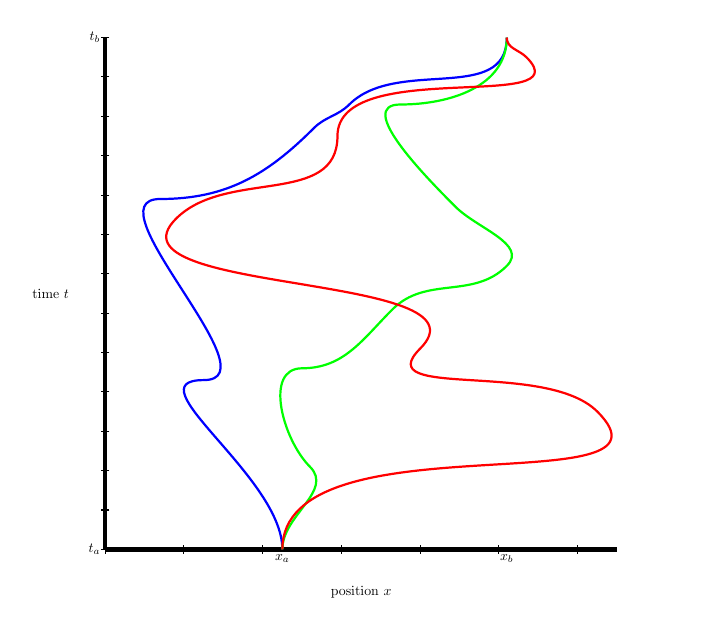
\begin{tikzpicture}[scale=0.5, every node/.style={transform shape}]
                \draw [ultra thick] [-] (0,13) -- coordinate (y axis mid) (0,0);
                \draw [ultra thick] [-] (0,0) -- coordinate (x axis mid) (13,0);
                \foreach \x in {0,2,...,13}
                    \draw (\x,3pt) -- (\x,-3pt);
                \foreach \y in {0,...,13}
                    \draw (3pt,\y) -- (-3pt,\y);
                \node[below=0.8cm] at (x axis mid) {position $x$};
                \node[left=0.8cm] at (y axis mid) {time $t$};
                \node [left] at (0,0) {$t_{a}$};
                \node [left] at (0,13) {$t_{b}$};
                \node [below] at (4.5,0) {$x_a$};
                \node [below] at (10.2,0) {$x_b$};
                \draw [-,thick, blue] (4.5,0) to [out=90,in=180] (2.5,4.3)
                        to [out=0,in=180] (1.4,8.9) to [out=0,in=-135] (5.3,10.7) 
                        to [out=45,in=225] (6.2,11.3) to [out=45,in=-90] (10.2,13);
                \draw [-,thick, green] (4.5,0) to [out=90,in=-45] (5.2,2.1)
                        to [out=135,in=180] (5.0,4.6) to [out=0,in=-135] (7.3,6.1) 
                        to [out=45,in=225] (10.2,7.2) to [out=45,in=-45] (8.9,8.7)
                        to [out=135,in=180] (7.5,11.3) to [out=0,in=-90] (10.2,13);
                \draw [-,thick, red] (4.5,0) to [out=90,in=-45] (12.5,3.5)
                        to [out=135,in=225] (8,5.1) to [out=45,in=-135] (1.8,8.4) 
                        to [out=45,in=270] (5.9,10.5) to [out=90,in=-45] (10.7,12.5)
                        to [out=135,in=-90] (10.2,13);
            \end{tikzpicture}
            \caption{Three of the infinitely many paths from $\left(x_a,t_a\right)$ to $\left(x_b,t_b\right)$ that contribute to the path integral.} 
            \label{fig:ExamplePathIntegrals}
        \end{figure}

        In the transition amplitude we integrate over an infinite number of paths, figure \ref{fig:ExamplePathIntegrals} shows three such paths that contribute to the path integral. The first step in calculating the path integral is to discretise time, this is shown in figure \ref{fig:TimeLattice} where we have discretised the green path in figure \ref{fig:ExamplePathIntegrals} onto a time lattice and we assume the particle travels along a straight line between the time sites.
        \begin{figure}
            \centering
            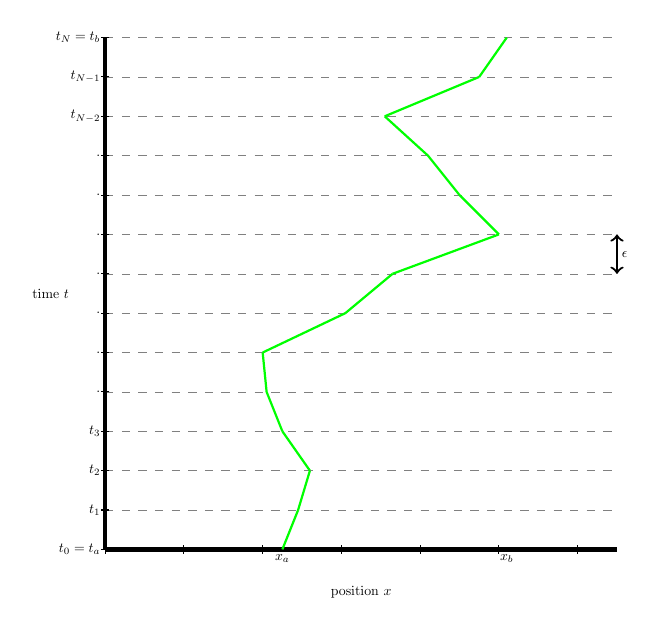
\begin{tikzpicture}[scale=0.5, every node/.style={transform shape}]
                
                \foreach \y in {0,...,13}{ \draw [help lines, dashed] (0,\y) -- (13,\y); }
                \draw [ultra thick] [-] (0,13) -- coordinate (y axis mid) (0,0);
                \draw [ultra thick] [-] (0,0) -- coordinate (x axis mid) (13,0);
                \foreach \x in {0,2,...,13}
                    \draw (\x,3pt) -- (\x,-3pt);
                \foreach \y in {0,...,13}
                    \draw (3pt,\y) -- (-3pt,\y);
                \node [left] at (0,0) {$t_{0}=t_{a}$};
                \node [left] at (0,1) {$t_{1}$};
                \node [left] at (0,2) {$t_{2}$};
                \node [left] at (0,3) {$t_{3}$};
                \node [left] at (0,4) {$.$};
                \node [left] at (0,5) {$.$};
                \node [left] at (0,6) {$.$};
                \node [left] at (0,7) {$.$};
                \node [left] at (0,8) {$.$};
                \node [left] at (0,9) {$.$};
                \node [left] at (0,10) {$.$};
                \node [left] at (0,11) {$t_{N-2}$};
                \node [left] at (0,12) {$t_{N-1}$};
                \node [left] at (0,13) {$t_{N}=t_{b}$};
                \node[below=0.8cm] at (x axis mid) {position $x$};
                \node[left=0.8cm] at (y axis mid) {time $t$};
                \draw [thick] [<->] (13,7) -- (13,8) ;
                \node [below=0.5cm] [right] at (13,8) {$\epsilon$};
                \draw [thick,green] (4.5,0) -- (4.9,1);
                \draw [thick,green] (4.9,1) -- (5.2,2);
                \draw [thick,green] (5.2,2) -- (4.5,3);
                \draw [thick,green] (4.5,3) -- (4.1,4);
                \draw [thick,green] (4.1,4) -- (4.0,5);
                \draw [thick,green] (4.0,5) -- (6.1,6);
                \draw [thick,green] (6.1,6) -- (7.3,7);
                \draw [thick,green] (7.3,7) -- (10,8);
                \draw [thick,green] (10,8) -- (9.0,9);
                \draw [thick,green] (9.0,9) -- (8.2,10);
                \draw [thick,green] (8.2,10) -- (7.1,11);
                \draw [thick,green] (7.1,11) -- (9.5,12);
                \draw [thick,green] (9.5,12) -- (10.2,13);
                \node [below] at (4.5,0) {$x_a$};
                \node [below] at (10.2,0) {$x_b$};
            \end{tikzpicture}
            \caption{Discretising time and a path from $\left(x_a,t_a\right)$ to $\left(x_b,t_b\right)$  onto a lattice of time spacing $\epsilon$.}
            \label{fig:TimeLattice}
        \end{figure}
        For each time site on the lattice $t_i$ we have a position $x_i = x\left(t_i\right)$ where $i=0,1,\dots,N$. We introduce the notation:
        \begin{equation}
            \label{eq:configuration}
            \bm{x}=\left(x_0,x_1,\dots,x_{N}\right)
        \end{equation}
        to denote a particular path on the lattice where each position coordinate has been specified and we refer to equation \ref{eq:configuration} as a \textit{configuration} on the lattice. In our notation for the labelling of the position eigenstates in equation \ref{eq:PathIntegral} we also have $x_b=x_{N}=x\left(t_{N}\right)$ and $x_a=x_0=x\left(t_0\right)$ in order to match with figure \ref{fig:TimeLattice}. $ \epsilon $ is the spacing between lattice sites and so $\epsilon = \frac{t_b-t_a}{N} = t_{i+1}-t_i$ and for $k=0,1,\dots,N$ we have $ t_k = t_a + k \epsilon $. In order to discretise the action in equation \ref{eq:MinkowskiAction} we approximate the derivative by a forward difference and the integral as a Riemann sum since we assume the particle is travelling on a straight line between lattice sites:
        
        \begin{equation}
            \label{eq:DiscreteMinkowskiAction}
            S_{M}\left(\bm{x}\right) = \sum_{i=0}^{N-1} \epsilon \left[\frac{1}{2}m\left(\frac{x_{i+1}-x_{i}}{\epsilon}\right)^{2} - V\left(x_i\right)\right].
        \end{equation}
        Since  for $i=1,2,\dots,N-1, -\infty < x_i < \infty$ we may define the integral measure in equation \ref{eq:PathIntegral} as:
        \begin{equation}
            \label{eq:IntegralMeasure}
            \int_{x_a}^{x_b} {\cal D} x \sim \prod_{n=1}^{N-1}\int_{-\infty}^{\infty}dx_n,
        \end{equation}
        which up to normalisation integrates over all possible routes through the lattice; so that for our discrete time lattice, the path integral is given by:
        \begin{equation}
            \label{eq:DiscretePathIntegral}
            Z_{ba} \sim \int^{+\infty}_{-\infty}\prod_{i=1}^{N-1}dx_i \exp{\left(\frac{i}{\hbar}S_M\left(\left\{x_i\right\}\right)\right)}.
        \end{equation}
        In the limit that $N\rightarrow \infty$ (or equivalently $\epsilon \rightarrow 0$) we recover (up to normalisation) equation \ref{eq:PathIntegral} from equation \ref{eq:DiscretePathIntegral} exactly. 


        In order to work with the discrete path integral we have one final step. We make a \textit{Wick rotation} into imaginary time; this is done via the substitution:
        \begin{equation}
            \label{eq:WickRotation}
            \tau = it.
        \end{equation}
        Applying this to the discretised theory developed above by defining $a=i\epsilon$, we now have a lattice in imaginary time, of lattice spacing $a$, substituting $a$ into equation \ref{eq:DiscreteMinkowskiAction}:
        \begin{align}
            \label{eq:DiscreteEuclideanAction1}
            S_M\left(\bm{x}\right) & = i\sum_{i=0}^{N-1} a \left[\frac{1}{2}m\left(\frac{x_{i+1}-x_{i}}{a}\right)^2 + V(x_i)\right] \\
            \label{eq:DiscreteEuclideanAction2} & = iS_E\left(\bm{x}\right),
        \end{align}
        where we have redefined the notation slightly so that $x_i=x\left(\tau_i\right)$ since we now have a lattice in imaginary time.
        The quantity
        \begin{equation}
            \label{eq:DiscreteEuclideanAction}
            S_{E}\left(\bm{x}\right) \equiv \sum_{i=0}^{N-1} a \left[\frac{1}{2}m\left(\frac{x_{i+1}-x_{i}}{a}\right)^2 + V(x_i)\right]
        \end{equation}
        is the discretised ``Euclidean'' action; it has this name because the effect of the Wick transformation is that it turns the Minkowski metric $ds_{M}$ on the coordinates $\left(x,y,z,t\right)$ into the Euclidean metric $ds_{E}$ on the coordinates $\left(x,y,z,\tau\right)$ and vice-versa:
        \begin{align}
            \label{eq:MinkowskiMetric} ds_{M}^{2} & = -dt^2 + dx^2 + dy^2 + dz^2 \\
            \label{eq:MetricTransform}            & = d\tau^2 + dx^2 + dy^2 + dz^2 \\
            \label{eq:EuclideanMetric}            & = ds_{E}^{2}.
        \end{align}
        Equation \ref{eq:DiscreteEuclideanAction2} is a very useful result since upon substitution into the discrete path integral we find:
        \begin{equation}
            \label{eq:DiscreteEuclideanPathIntegral}
            Z_{ba} \sim \int^{+\infty}_{-\infty}\prod_{i=1}^{N-1}dx_i \exp{\left(-\frac{1}{\hbar}S_{E}\left(\left\{x_i\right\}\right)\right)}
        \end{equation}
        which is known as the discrete euclidean path integral and will converge since the integrand is now exponentially suppressed. We will impose periodic boundary conditions by identifying the first and last lattice sites (i.e. take $x_b=x_a$) and then integrate over that site, which can be quantified through: 
        \begin{align}
            \label{eq:partWithBoundaryConditions}
            Z & = \int dx_a \int dx_b \delta\left(x_b-x_a\right)Z_{ba} \\
              & = \int^{+\infty}_{-\infty}\prod_{i=0}^{N-1}dx_i \exp{\left(-\frac{1}{\hbar}S_{E}\left(\left\{x_i\right\}\right)\right)}.
        \end{align}
        We have the standard result from statistical physics that for a system with a fixed number $N$ of continuous degrees of freedom labelled by $x_i$ for $i=0,1,\dots N-1$ then the canonical partition function is given by:
        \begin{equation}
            \label{eq:PartitionFunction}
            \mathcal{Z} \sim \int_{-\infty}^{+\infty}\prod_{i=0}^{N-1}dx_{i}\exp{\left(-\beta H\left(\left\{x_i\right\}\right)\right)},
        \end{equation}
        with $\beta=\frac{1}{k_{B}T}$ where $T$ is the system temperature and $k_{B}$ is the Boltzmann constant. Comparing equation \ref{eq:partWithBoundaryConditions} to equation \ref{eq:PartitionFunction} we can see that the discretised Euclidean path integral is a classical canonical partition function on a system with $N$ degrees of freedom, provided that we take:
        \begin{equation}
            \label{ActionToHamiltonian}
            \frac{1}{\hbar}S_{E}\left(\left\{x_{i}\right\}\right) = \beta H\left(\left\{x_{i}\right\}\right),
        \end{equation}
        and impose periodic boundary conditions. We then have a Boltzmann factor given by $\exp{\left(-\frac{1}{\hbar}S_{E}\left(\left\{x_{i}\right\}\right)\right)}$. So in summary we now have a classical interpretation of our quantum calculation of the path integral; our lattice is essentially a one dimensional crystal of size $N$ at temperature $T$ with a continuous variable $x_i$ at each crystal site, and its Hamiltonian is given by $S_E\left(\left\{x_i\right\}\right)$.

        It is interesting to note that in quantum mechanics, due to the uncertainty principle $\Delta x\Delta p \geq \frac{\hbar}{2}$, $\hbar$ provides a measure of quantum fluctuations in our system. As $\hbar \rightarrow 0$ we recover classical physics and in this limit the only path in the path integral that contributes to the transition amplitude is the classical one. On the other hand, in statistical mechanics $T$ provides a measure of statistical fluctuations in our system, and in the limit that $T \rightarrow 0$ these fluctuations go to zero. Hence taking the limit that $\hbar \rightarrow 0$ and $T \rightarrow 0$ we see statistical mechanics on a (real) crystal lattice is equivalent quantum mechanics in imaginary time.



\section{Methods}
    \subsection{Monte Carlo Methods}
    Monte Carlo methods provide a way of numerically evaluating integrals where the error is independent of the dimensionality of the integral. For the purposes of our work we will be interested in estimating expectation values of functions (which are the observables of our statistical system) $\phi\left(X\right)$ of some d-dimensional random variable $X$ under some probability distribution with density function $f\left(\bm{x}\right)$:
    \begin{equation}
        \label{eq:expectation}
        \langle \phi\left(X\right) \rangle = \int \prod_{i=1}^{d}{dx_i}f\left(\bm{x}\right)\phi\left(\bm{x}\right),
    \end{equation}
    since this takes the form of the path integral we wish to calculate, where $\bm{x}$ correspond to the configurations on the lattice, $f\left(\bm{x}\right)$ the canonical distribution and $\phi\left(\bm{x}\right)$ some function on the lattice such as mean position. In order to estimate the expectation value/integral we approximate the expectation as a sample mean on some finite set of $M$ samples of $X$ as (we will refer to this as the \textit{Monte Carlo estimate}):
    \begin{equation}
        \label{eq:montecarloestimate}
        \langle\phi\left(X\right)\rangle \approx \frac{1}{M} \sum_{n=1}^{M}\phi\left(\bm{x}_n\right).
    \end{equation}
    It can be shown that the error in \ref{eq:montecarloestimate} is always $\mathcal{O}\left(1/\sqrt{M}\right)$ independent of the dimension of the integral, and that the Monte method wins over quadrature methods (traditional numerical integration schemes) in terms of computational cost vs. accuracy for $d>3$ \cite{gattringer_lang_2013}.
    It is now just a question of how to choose the samples $\bm{x}_n$ to get a expectation value with a small error. From the form of equation \ref{eq:expectation} drawing uniform samples from the support of $f$ is clearly unwise, since this would give equal weight to contributions to our approximation of the expectation value for samples that are very unlikely to be realised by the random variable $X$ under the density function $f$ as those which are very likely to be realised. We therefore choose to draw samples according to the distribution of $X$, this is known as \textit{importance sampling}. In order to draw samples according to a probability distribution we use a \textit{Markov chain} which for our purposes can be defined as a sequence of random variables (samples) for which the probability of the next random variable in the sequence taking on a particular value depends only on the current random variable, we will denote this probability by $P_M\left(\bm{x}\rightarrow \bm{x}'\right)$. By starting from some arbitrary state (which in our simulation is a configuration) through the stochastic sequence of configurations we will eventually end up sampling from the desired equilibrium distribution with density function $f\left(\bm{x}\right)$. This idea of a \textit{Markov Chain Monte Carlo} method was first introduced by Metropolis et al. in \cite{metropolis_rosenbluth_rosenbluth_teller_teller_1953} via the Metropolis algorithm. Hybrid Monte Carlo is a method for constructing such a Markov chain and it is discussed in the next section. 

    A Markov chain will converge on a distribution with density function $P\left(\bm{x}\right)$ provided the chain is ergodic and obeys detailed balance. Ergodicity is the condition that any sample that can be realised under the probability distribution can be reached through the Markov chain and the detailed balance condition is given by: 
    \begin{equation}
        \label{eq:detailedbalance}
        P\left(\bm{x}\right)P_M\left(\bm{x}\rightarrow \bm{x}'\right)=P\left(\bm{x}'\right)P_M\left(\bm{x}'\rightarrow \bm{x}\right).
    \end{equation}
    During an actual simulation, one only starts to calculate the values of observables via equation \ref{eq:montecarloestimate} after an equilibration period, this is due to the fact that initially samples will not be drawn according to the correct probability distribution and it is only once the Markov chain has converged that they will. 

    We may consider our Monte Carlo simulation as consisting of three main stages. First to start the simulation we provide an initial configuration to begin the chain. We then have to perform a sufficient number of updates/steps of the chain such that we are drawing from the correct distribution, which in our case is the canonical distribution for our statistical system. Once we are at equilibrium we may compute the values of any observables on any configuration and use them to calculate the Monte Carlo estimate. In order to provide an initial lattice configuration we found that after some experimentation, a reasonable method was to provide a so called \textit{hot start} by uniformly distributing the position values of the lattice sites on the interval $\left[-1,1\right]$. In order to determine when and if samples are being drawn from the equilibrium distribution one can observe the evolution of some set of observables, for example position, and see when these values begin to converge. This method has potential issues in that there are the possibilities of \textit{metastable states} \cite{sokal_1997} for which it may seem as if the system has reached equilibrium, when in fact it is sampling from region of the configuration space for which it is metastable but will not remain indefinitely. This issue will arise for the case of the anharmonic oscillator, where the possibility of the particle getting ``stuck'' in one well can lead to Monte Carlo estimates on $\langle x \rangle$ being non-zero for a symmetric well about zero. However, in this case we are able to identify when this metastability has occurred, since by symmetry we know the true answer. Once we have achieved equilibrium we are able to evaluate observables via the configurations, due to the possibility of correlations between samples in the Markov chain this is not entirely trivial, and the analysis of recorded data is discussed at the end of this chapter.



    \subsection{Hybrid Monte Carlo}
        \subsubsection{Hamiltonian Dynamics}
            \label{sec:HamiltonianDynamics}
            Due to the fundamental importance of Hamiltonian dynamics in the Hybrid-Monte Carlo algorithm in this section we provide a quick review of Hamilton's equations and explain the numerical method used to integrate these equations so that they may be used in computational simulations.

            Hamiltonian Dynamics enables us to solve the time evolution of a system of canonical coordinates $\left(\bm{q},\bm{p}\right)$ where the $d$-dimensional $\bm{q}=\left(q_1,q_2,\dots,q_d\right)$ and $\bm{p}=\left(p_1,p_2,\dots,p_d\right)$ vectors are called \textit{position} and \textit{momentum} respectively. The system is then characterised by a Hamiltonian function $H\left(\bm{q},\bm{p}\right)$ on the $2d$-dimensional \textit{phase space} occupied by the $\left(\bm{q},\bm{p}\right)$ vectors. \textbf{Hamilton's equations}:
            \begin{align}
                \label{eq:HamiltonsEquation1} \frac{dq_i}{dt} & = \frac{\partial H}{\partial p_i} \\
                \label{eq:HamiltonsEquation2} \frac{dp_i}{dt} & = -\frac{\partial H}{\partial q_i}
            \end{align}
            for $i = 1, 2, \dots d$, provide the time evolution of the vectors $\bm{q}$ and $\bm{p}$, so that if the state of the system is $\left(\bm{q},\bm{p}\right)$ at time $t$ then Hamilton's equations give a mapping $T_s$ to the state $\left(\bm{q}',\bm{p}'\right)$ at time $t+s$.  We will see in section \ref{sec:SamplingAndTheHamiltonian} for the purposes of the implementing the HMC algorithm we may assume that the Hamiltonian is of the form:
            \begin{equation}
                \label{eq:HamiltonianUPlusK}
                H\left(\bm{q},\bm{p}\right) = U\left(\bm{q}\right) + K\left(\bm{p}\right),
            \end{equation}
            Where $U\left(\bm{q}\right)$ and $K\left(\bm{p}\right)$ are known as the \textit{potential} and \textit{kinetic} terms respectively. Equations \ref{eq:HamiltonsEquation1} and \ref{eq:HamiltonsEquation2} then become:
            \begin{align}
                \label{eq:HamiltonsEquation1K} \frac{dq_i}{dt} & = \frac{\partial K}{\partial p_i} \\
                \label{eq:HamiltonsEquation2T} \frac{dp_i}{dt} & = -\frac{\partial U}{\partial q_i}.
            \end{align}

            Since we intend to use the solutions to Hamilton's equations in the HMC simulation we need to find a way of integrating them numerically; in \cite{neal_2011} it is argued that a successful method for this is \textit{leapfrog integration}. In the leapfrog method to make the small time step $\epsilon$ from $t$ to $t+\epsilon$ in position and momentum we use the equations:
            \begin{align}
                \label{eq:LeapFrogEq1} p_i\left(t+\epsilon/2\right) & = p_i\left(t\right) + \epsilon/2\frac{dp_i}{dt}\left(t\right)\\ 
                 & = p_i\left(t\right) - \epsilon/2\frac{\partial U}{\partial q_i}\left(\bm{q}\left(t\right)\right), \\
                \label{eq:LeapFrogEq2}q_i\left(t+\epsilon\right) & = q_i\left(t\right) + \epsilon\frac{dq_i}{dt}\left(t+\epsilon/2\right) \\
                &  = q_i\left(t\right) + \epsilon\frac{\partial K}{\partial p_i}\left(\bm{p}\left(t+\epsilon/2\right)\right), \\
                \label{eq:LeapFrogEq3}p_i\left(t+\epsilon\right) & = p_i\left(t+\epsilon/2\right) + \epsilon/2\frac{dp_i}{dt}\left(t+\epsilon/2\right) \\
                & = p_i\left(t+\epsilon/2\right) - \epsilon/2\frac{\partial U}{\partial q_i}\left(\bm{q}\left(t+\epsilon\right)\right),
            \end{align}
            where in the second equality in each step we have made the substitution for Hamilton's equations.
            In equation \ref{eq:LeapFrogEq1} we begin with a half step in each momentum component to go from $t$ to $t+\epsilon/2$. Using the half stepped momenta we then do a full step from $t$ to $t+\epsilon$ in each position component in equation \ref{eq:LeapFrogEq2}. We end in equation \ref{eq:LeapFrogEq3} with a second half step in the momentum components to go from $t+\epsilon/2$ to $t+\epsilon$ using the updated position components. Iterating this process we do as many steps of size $\epsilon$ as we like.

            This generalises to making $l$ steps in position and momentum and we can combine any two half steps in momentum that follow one another to simplify the algorithm which is often more convenient for computation purposes. Starting at $t=0$:
            \begin{enumerate}
                \item We begin with a half step in momentum:
                \begin{equation}
                    \label{eq:MomentumInitialHalfStep}
                    p_i\left(\epsilon/2\right) = p_i\left(0\right) - \epsilon/2\frac{\partial U}{\partial q_i}\left(\bm{q}\left(0\right)\right),
                \end{equation}
                and a full step in position:
                \begin{equation}
                    \label{eq:PositionInitialStep}
                    q_i\left(\epsilon\right) = q_i\left(0\right) + \epsilon\frac{\partial K}{\partial p_i}\left(\bm{p}\left(\epsilon/2\right)\right).
                \end{equation}
                \item Then make $l-1$ alternating steps in momentum and position:
                \begin{equation}
                    \label{eq:MomentumFullStep}
                    p_i\left(n\epsilon+\epsilon/2\right) = p_i\left(n\epsilon-\epsilon/2\right) - \epsilon\frac{\partial U}{\partial q_i}\left(\bm{q}\left(n\epsilon\right)\right),
                \end{equation}
                \begin{equation}
                    \label{eq:PositionFullStep}
                    q_i\left(n\epsilon+\epsilon\right) = q_i\left(n\epsilon\right) + \epsilon\frac{\partial K}{\partial p_i}\left(\bm{p}\left(n\epsilon+\epsilon/2\right)\right),
                \end{equation}
                for $n = 1, \dots , l-1$.
                \item Then a final half step in momentum:
                \begin{equation}
                    \label{eq:Momnetum}
                    p_i\left(l\epsilon\right) = p_i\left(l\epsilon-\epsilon/2\right) - \epsilon/2\frac{\partial U}{\partial q_i}\left(\bm{q}\left(l\epsilon\right)\right).
                \end{equation}
            \end{enumerate}
            The reasoning for the name \textit{leapfrog} becomes apparent here since apart from the initial and final half steps in momentum, the momentum and position values are used alternatively to calculate the position and momentum respectively at the next step and the variables ``leap'' over one another at on offset of $\epsilon/2$. 

            An important feature of the leap frog integration scheme that makes it applicable to HMC is that it preserves volume in phase space exactly, which we will see leads to detailed balance. For Hamiltonian dynamics in continuous time, preservation of volume in phase space is known as Louville's theorem and its proof is given in \cite{goldstein_poole_safko_2014}. For the discrete dynamics integrated via the leap frog scheme we can easily verify that volume preservation is still the case. First let us define the mappings $T_q\left(\epsilon\right): \left(\bm{q},\bm{p}\right) \rightarrow \left(\bm{q}',\bm{p}'\right) $ and $T_p\left(\epsilon\right): \left(\bm{q},\bm{p}\right) \rightarrow \left(\bm{q}',\bm{p}'\right)$ on phase space such that:
            \begin{align}
                \label{eq:psMap1}
                T_q\left(\epsilon\right)\begin{pmatrix} \bm{q} \\ \bm{p} \end{pmatrix} & = \begin{pmatrix} \bm{q} +\epsilon \underline{\nabla}_pK\left(\bm{p}\right) \\ \bm{p} \end{pmatrix}, \\
                \label{eq:psMap2}
                T_p\left(\epsilon\right)\begin{pmatrix} \bm{q} \\ \bm{p} \end{pmatrix} & = \begin{pmatrix} \bm{q} \\ \bm{p} - \epsilon \underline{\nabla}_qU\left(\bm{q}\right) \end{pmatrix},
            \end{align}
            then (with a slight abuse of notation) the Jacobians of these mappings will be of the form:
            \begin{equation}
                J = \det\begin{pmatrix}\frac{\partial q_i'}{\partial q_j} & \frac{\partial q_i'}{\partial p_j} \\ \frac{\partial p_i'}{\partial q_j} & \frac{\partial p_i'}{\partial p_j} \end{pmatrix}
            \end{equation}
            so that:
            \begin{align}
            J_q& =\det\begin{pmatrix} \delta_{ij} & \epsilon\partial_{p_i}\partial_{p_j}K\left(\bm{p}\right) \\ 0 & \delta_{ij} \end{pmatrix} = 1 \\
            J_p& =\det\begin{pmatrix} \delta_{ij} &  0  \\ -\epsilon\partial_{q_i}\partial_{q_j}U\left(\bm{q}\right) & \delta_{ij} \end{pmatrix} = 1.
            \end{align}
            For a single step of size $\epsilon$ the leap frog algorithm equations \ref{eq:LeapFrogEq1}, \ref{eq:LeapFrogEq2} and \ref{eq:LeapFrogEq3} define a mapping on phase space $T\left(\epsilon\right): \left(\bm{q}\left(t\right),\bm{p}\left(t\right)\right) \rightarrow \left(\bm{q}\left(t+\epsilon\right),\bm{p}\left(t+\epsilon\right)\right)$ that can be written using the mappings given above as:
            \begin{equation}
                T\left(\epsilon\right)=T_p\left(\epsilon/2\right)T_q\left(\epsilon\right)T_p\left(\epsilon/2\right).
            \end{equation}
            Since each map in the composition on the right hand side of this equation has a Jacobian of $1$ we have that the Jacobian of $T\left(\epsilon\right)$ is $1$. For the total trajectory which consists of $l$ steps we may write the mapping that via leapfrog integration takes us from the start to the end of the trajectory as:
            \begin{equation}
                \text{traj}\left(\epsilon,l\right) = \left(T\left(\epsilon\right)\right)^l
            \end{equation}
            which of course also a Jacobian of $1$ since each mapping in the composition has Jacobian $1$ and hence the leapfrog integration preserves volume on the phase space since as a mapping its Jacobian is $1$. We will return to this argument in section \ref{sec:Tempering} where we will show that the leap frog integration scheme preserves volume even for the case of tempered dynamics. 
            
            It is also obvious that the leapfrog integration scheme provides reversible dynamics; by negating the momenta at the end of a trajectory and applying the equations a second time we will return to the initial point in phase space. Negating the momenta at the end of a leapfrog trajectory will also preserve the volume.



        

        \subsubsection{Sampling and the Hamiltonian}
            \label{sec:SamplingAndTheHamiltonian}
            For a physical system in thermodynamic equilibrium with a fixed number of degrees of freedom and with energy function $E\left(\bm{x}\right)$, where the vector $\bm{x} = \left(x_{1},x_{2},\dots,x_{d}\right)$ denotes the state of the system that depends on $d$ variables, the canonical Boltzmann distribution (probability density function for the states of the system) in units where $k_b=1$ is given by:
            \begin{equation}
                \label{eq:BoltzmannDistribution}
                P\left(\bm{x}\right) = \frac{1}{\mathcal{Z}} \exp{\left(-\frac{E\left(\bm{x}\right)}{T} \right)},
            \end{equation}
            where $\mathcal{Z}$ is the canonical partition function for the system which provides the normalisation and is given by 
            \begin{equation}
                \label{eq:JointPartitionFunction}
                \mathcal{Z} = \int\prod_{i=1}^{d}dx_{i} \exp{\left(-\frac{E\left(\bm{x}\right)}{T} \right)}.
            \end{equation}
            Alternatively any probability distribution $P\left(\bm{x}\right)$ can be constructed as the Boltzmann distribution for the energy function $ E\left(\bm{x}\right) = -T\left(\log{P\left(\bm{x}\right)} + \log{\mathcal{Z}}\right)$ for some choice of $T$ and $\mathcal{Z}$. 

            A Hamiltonian of the form $H\left(\bm{q},\bm{p}\right)=U\left(\bm{q}\right)+K\left(\bm{p}\right)$ is an energy function on the $2d$-dimensional phase space given by position and momentum $\left(\bm{q},\bm{p}\right)$, with $\bm{q} = \left(q_{1},q_{2},\dots,q_{d}\right)$ and $\bm{p} = \left(p_{1},p_{2},\dots,p_{d}\right)$. We may define a Boltzmann distribution on those variables by:
            \begin{equation}
                \label{eq:BoltzmannDistributionXP}
                P\left(\bm{q},\bm{p}\right) = \frac{1}{\mathcal{Z}}\exp{\left(-\frac{H\left(\bm{q},\bm{p}\right)}{T} \right)},
            \end{equation}
            with 
            \begin{equation}
                \mathcal{Z} = \int\prod_{i=1}^{d}dx_{i}dp_{i} \exp{\left(\frac{-H\left(\bm{q},\bm{p}\right)}{T}\right)}
            \end{equation}
            Then, if $H\left(\bm{q},\bm{p}\right) = U\left(\bm{q}\right) + K\left(\bm{p}\right)$ this factorises as:
            \begin{equation}
                \label{eq:BoltzmannDistributionXPFactorised}
                P\left(\bm{q},\bm{p}\right) = \frac{1}{\mathcal{Z}_U}\exp{\left(-\frac{U\left(\bm{q}\right)}{T} \right)}\frac{1}{\mathcal{Z}_K}\exp{\left(-\frac{K\left(\bm{p}\right)}{T} \right)} = P\left(\bm{q}\right) P\left(\bm{p}\right),
            \end{equation}
            so the variables $\bm{q}$ and $\bm{p}$ and their respective probability distributions are independent with energy functions $U\left(\bm{q}\right)$ and $K\left(\bm{p}\right)$. This means that in order to sample $\bm{q}$ from the marginal distribution $P\left(\bm{q}\right)$ we can sample from the joint distribution $P\left(\bm{q},\bm{p}\right)$ and disregard the $\bm{p}$. 

            In the HMC algorithm we employ Hamiltonian dynamics to sample from the joint distribution $P\left(\bm{q},\bm{p}\right)$. Therefore, if we have some probability distribution $P\left(\bm{x}\right)$ for states $\bm{x}$ we wish to sample, we may through equation \ref{eq:BoltzmannDistribution} define an energy function $E\left(\bm{x}\right)$ for that distribution. We then define $\bm{q}\equiv\bm{x}$ and $U\left(\bm{q}\right) \equiv E\left(\bm{x}\right)$, introduce ``fictitious momenta'' $\bm{p}$ and define a kinetic energy $K\left(\bm{p}\right)$ and the Hamiltonian $H\left(\bm{q},\bm{p}\right) = U\left(\bm{q}\right) + K\left(\bm{p}\right)$. Running the HMC algorithm generates samples according to the distribution given by equation \ref{eq:BoltzmannDistributionXP}, but by the factorization in equation \ref{eq:BoltzmannDistributionXPFactorised} this gives samples of $\bm{x}$ according to our original distribution $P\left(\bm{x}\right)$. In the HMC algorithm, we think of the variables of interest $\bm{x}$ as position $\bm{q}$ with conjugate momenta $\bm{p}$ which of course matches up nicely in physical applications where we are actually sampling position, although the algorithm is equally applicable in non-physical cases.

            Since the fictitious momenta $\bm{p}$ are introduced artificially, we need to choose their probability distribution $P\left(\bm{p}\right)$ by specifying the kinetic energy function $K\left(\bm{p}\right)$. For the purposes of our work we may take:
            \begin{equation}
                \label{eq:HMCQuadraticKineticEnergy}
                K\left(\bm{p}\right) = \sum_{i=1}^{d}\frac{p_i^2}{2}
            \end{equation}
            and $T=1$ from now on.

            \subsubsection{Steps of the HMC Algorithm}
            Here we will outline the main steps of the HMC algorithm then give a more detailed explanation of each stage and its implementation. The two key steps are \ref{en:HMCStep1} and \ref{en:HMCStep2}. In step \ref{en:HMCStep1} momentum is changed, where as in step \ref{en:HMCStep2} may change position and momentum. The canonical joint distribution for $\left(\bm{q},\bm{p}\right)$ is left invariant in both steps, and therefore is also invariant under their combination. The steps of the algorithm are:
            \begin{enumerate}
                \setcounter{enumi}{-1}
                \item \label{en:HMCStep0} Provide an initial sample $\bm{q}$
                \item \label{en:HMCStep1} Generate $\bm{p}$ from the multivariate Gaussian Distribution $\mathcal{N}\left(\bm{0},I_{d\times d}\right)$ 
                \item \label{en:HMCStep2} Evolve the variables from $\left(\bm{q},\bm{p}\right)$ to $\left(\bm{q'},\bm{p}'\right)$ by simulating Hamiltonian dynamics for $l$ steps of size $\epsilon$ and negating the momentum variables at the end of the trajectory. Accept the proposed state $\left(\bm{q}',\bm{p}'\right)$ as the next state in the Markov chain with probability:
                        \begin{equation*}
                            \min{\left[1,\exp{\left(-H_{HMC}\left(\bm{q}',\bm{p}'\right)+ \allowbreak H_{HMC}\left(\bm{q},\bm{p}\right)\right)}\right]}
                        \end{equation*}
                        If proposed state rejected, record current state $\bm{q}$ as sample (i.e. state started with), if successful set current state to proposed state $\bm{q}$ = $\bm{q}'$ and record it as a sample.
                \item \label{en:HMCStep5} Return to step \ref{en:HMCStep1} with $\bm{q}$.
            \end{enumerate}

            In step \ref{en:HMCStep0} we provide an initial state. This can be chosen or generated randomly, however, since we normally disregard the samples generated in the early HMC iterations as discussed above this choice is not critical. 

            In step \ref{en:HMCStep1} we draw the fictitious momenta according to their probability distribution. The choice of kinetic energy in equation \ref{eq:HMCQuadraticKineticEnergy} and the form of equation \ref{eq:BoltzmannDistribution} means that:
            \begin{align}
                \label{eq:KineticBoltzmannDistribution}
                P\left(\bm{p}\right) & = \frac{1}{Z_K}\exp{\left(-\sum_{i=1}^{d}\frac{p_i^2}{2}\right)} \\
                                     & = \prod_{i=1}^d\frac{1}{\sqrt{2\pi}} \exp{\left(-\frac{p_i^2}{2}\right)} \\
                                     & = \prod_{i=1}^dP\left(p_i\right)
            \end{align}
            where each $P\left(p_i\right)$ is a Gaussian distribution of mean $0$ and variance $1$. So the $d$ momentum variables are independent with each component $p_i$ of $\bm{p}$ drawn from a Gaussian $\mathcal{N}{\left(0,1\right)}$, so we draw $\bm{p}$ from a multivariate Gaussian distribution of mean $\bm{0}$ and covariance $I_{d\times d}$. In this step $\bm{q}$ is not changed, and $\bm{p}$ gets drawn from the it's correct conditional distribution given $\bm{q}$ which is it's marginal distribution by the above independence so the canonical joint distribution is left invariant.

            In step \ref{en:HMCStep2} we evolve the variables $\left(\bm{q},\bm{p}\right)$ by integrating Hamilton's equations. In order to implement this in a computer simulation we use the leapfrog method described in section \ref{sec:HamiltonianDynamics}. We have a choice of the number of time steps $l$ and their size $\epsilon$; it is common practice in HMC to choose $\epsilon$ and $l$ such that $l\epsilon=1$. At the end of the trajectory, negating the momentum variables makes the Metropolis proposal symmetric, which is needed for the acceptance probability to remain valid. However, in practice since $K\left(\bm{p}\right)=K\left(-\bm{p}\right)$ and the momentum is replaced anyway in the next iteration, there is no need for the negation. We accept or reject the proposed state with a probability given by:
            \begin{equation}
                \label{eq:HMCMetropolisUpdate}
                P\left(\bm{q}',\bm{p}',\bm{q},\bm{p}\right) = \min{\left[1,\exp{\left(-H_{HMC}\left(\bm{q}',\bm{p}'\right)+ \allowbreak H_{HMC}\left(\bm{q},\bm{p}\right)\right)}\right]},
            \end{equation}
            which is known as a \textit{Metropolis update}. The interpretation of \ref{eq:HMCMetropolisUpdate} is that if the Hamiltonian decreases (or stays constant) as a result of moving to the proposed state the update is accepted with certainty. However, if the Hamiltonian increases as a result of the moving to the proposed state, the proposal is accepted with a probability that decreases for larger increases in the Hamiltonian. If the state is accepted then it becomes the current state state i.e. $\bm{q} = \bm{q}'$, otherwise the current state remains as it was in step \ref{en:HMCStep1}. In either case we then record the current state as a sample and return to step \ref{en:HMCStep1} with the current state $\bm{q}$.

            From the Metropolis update in equation \ref{eq:HMCMetropolisUpdate} we can show that for smaller value of $\epsilon$ and larger $l$ (i.e. smaller time steps and more of them) the probability of accepting an update approaches unity. To see this note that as $\epsilon \rightarrow 0$ and $l \rightarrow \infty$ the leap frog method approaches an exact integration of Hamilton's equations. It is easily shown that for continuous time the Hamiltonian is a conserved quantity:
            \begin{align}
            \frac{dH}{dt}=\sum_{i=1}^{d}\left[\frac{dq_i}{dt}\frac{\partial H}{\partial q_i}+\frac{dp_i}{dt}\frac{\partial H}{\partial p_i}\right]=\sum_{i=1}^{d}\left[\frac{\partial H}{\partial p_i}\frac{\partial H}{\partial q_i}-\frac{\partial H}{\partial q_i}\frac{\partial H}{\partial p_i}\right]=0
            \end{align}
            where in the second equality we have used Hamilton's equations. Therefore as $\epsilon \rightarrow 0$ and $l\rightarrow \infty$, $H_{HMC}\left(\bm{q},\bm{p}\right) \rightarrow H_{HMC}\left(\bm{q}',\bm{p}'\right)$ and so the probability of accepting a state is always $1$.   

            As $\epsilon$ decreases $l$ increases provided $l\epsilon$ is kept fixed, therefore more steps and hence a larger computational cost is required for proposal states with smaller $\epsilon$ in the trajectory. Conversely if we have a fixed computation time, then for smaller $\epsilon$ we will generate less proposals with a higher acceptance rate and hence our the error in the Monte Carlo estimate on any observable will be larger. It is shown in \cite{beskos_pillai_roberts_sanz-serna_stuart_2013} that an acceptance rate of $\sim 65.1\%$ provides an optimal balance between the cost of generating proposals and the total number of samples.

            HMC will be typically ergodic \cite{neal_2011} however proving ergodicity is highly non-trivial, we will therefore assume that ergodicity of the HMC algorithm holds for our simulation and refer the reader to the mathematical literature on the subject such as \cite{bou-rabee_sanz-serna_2017}, \cite{durmus_moulines_saksman} and \cite{livingstone_betancourt_byrne_girolami} as justification.

            We can however show that HMC obeys detailed balance using a proof similar to that given in \cite{duane_kennedy_pendleton_roweth_1987}. In order to do this we will (for notational simplicity) adopt the field theory notation and set $\bm{q}\rightarrow \phi$ and $\bm{p}\rightarrow \pi$ and redefine the canonical distribution in equation \ref{eq:BoltzmannDistributionXP} as $P\left(\bm{q},\bm{p}\right) \rightarrow p\left(\phi,\pi\right)$ where we are using a lower case $p$ to emphasise the fact we are dealing with a probability density. $p\left(\phi,\pi\right)d\phi d\pi$ is then the probability of being in the volume given by the intervals $\left[\phi,\phi+d\phi\right]$ and  $\left[\pi,\pi+d\pi\right]$ so if $P\left(\left(\phi,\pi\right)\rightarrow\left(\phi',\pi'\right)\right)$ is the probability of moving from $\left(\phi,\pi\right)$ to $\left(\phi',\pi'\right)$ the detailed balance condition is given by:
            \begin{equation}
                \label{eq:HMCDetailedBalance}
                d\phi d\pi p\left(\phi,\pi\right) P\left(\left(\phi,\pi\right)\rightarrow\left(\phi',\pi'\right)\right) = d\phi' d\pi' p\left(\phi',\pi'\right) P\left(\left(\phi',\pi'\right)\rightarrow\left(\phi,\pi\right)\right).
            \end{equation}
            We have shown preservation of volume in phase space for the leapfrog method, so that $d\phi d\pi = d\phi' d\pi'$. We may decompose the second factor in the LHS of equation \ref{eq:HMCDetailedBalance} as:
            \begin{equation}
                P\left(\left(\phi,\pi\right) \rightarrow \left(\phi',\pi'\right)\right) = P_{H}\left(\left(\phi,\pi\right) \rightarrow \left(\phi',\pi'\right)\right)P_{A}\left(\left(\phi,\pi\right)\rightarrow \left(\phi',\pi'\right)\right)
            \end{equation}
            where $P_{H}$ is the probability of proposing the update under the Hamiltonian $H$ and $P_A$ is the probability of actually accepting that move. By the fact that leapfrog is reversible we have that
            \begin{equation}
                P_{H}\left(\left(\phi,\pi\right) \rightarrow \left(\phi',\pi'\right)\right) =  P_{H}\left(\left(\phi',-\pi'\right) \rightarrow \left(\phi,-\pi\right)\right)
            \end{equation}
            and since we are using the metropolis update step
            \begin{equation}
                P_{A}\left(\left(\phi,\pi\right)\rightarrow \left(\phi',\pi'\right)\right) = \min\left[1,\exp\left(-\left(H\left(\phi',\pi'\right)-H\left(\phi,\pi\right)\right)\right)\right].
            \end{equation}
            Starting from the LHS of equation \ref{eq:HMCDetailedBalance} we get that:
            \begin{align}
                & d\phi d\pi p\left(\phi,\pi\right) P\left(\left(\phi,\pi\right)\rightarrow\left(\phi',\pi'\right)\right) \\
                 & = d\phi d\pi \frac{1}{\mathcal{Z}}e^{-H\left(\phi,\pi\right)}P_{H}\left(\left(\phi,\pi\right) \rightarrow \left(\phi',\pi'\right)\right)\min{\left[1,e^{\left(-\left(H\left(\phi',\pi'\right)-H\left(\phi,\pi\right)\right)\right)}\right]}\\ 
                 & = d\phi d\pi \frac{1}{\mathcal{Z}}e^{-H\left(\phi',\pi'\right)}P_{H}\left(\left(\phi',-\pi'\right) \rightarrow \left(\phi,-\pi\right)\right)\min{\left[e^{\left(-\left(H\left(\phi,\pi\right)-H\left(\phi',\pi'\right)\right)\right)},1\right]}\\
                 & = d\phi d\left(-\pi\right) \frac{1}{\mathcal{Z}}e^{-H\left(\phi',\pi'\right)}P_{H}\left(\left(\phi',-\pi'\right) \rightarrow \left(\phi,\pi\right)\right)\min\left[1,e^{\left(-\left(H\left(\phi,-\pi\right)-H\left(\phi',\pi'\right)\right)\right)}\right]\\
                 & = d\phi d\pi \frac{1}{\mathcal{Z}}e^{-H\left(\phi',\pi'\right)}P_{H}\left(\left(\phi',-\pi'\right) \rightarrow \left(\phi,\pi\right)\right)\min\left[1,e^{\left(-\left(H\left(\phi,-\pi\right)-H\left(\phi',\pi'\right)\right)\right)}\right]\\
                 & = d\phi' d\pi' \frac{1}{\mathcal{Z}}e^{-H\left(\phi',\pi'\right)}P_{H}\left(\left(\phi',-\pi'\right) \rightarrow \left(\phi,\pi\right)\right)\min\left[1,e^{\left(-\left(H\left(\phi,-\pi\right)-H\left(\phi',\pi'\right)\right)\right)}\right]\\ 
                 & = d\phi' d\left(-\pi'\right) \frac{1}{\mathcal{Z}}e^{-H\left(\phi',-\pi'\right)}P_{H}\left(\left(\phi',\pi'\right) \rightarrow \left(\phi,\pi\right)\right)\min\left[1,e^{\left(-\left(H\left(\phi,-\pi\right)-H\left(\phi',-\pi'\right)\right)\right)}\right]\\
                 & = d\phi' d\pi' \frac{1}{\mathcal{Z}}e^{-H\left(\phi',\pi'\right)}P_{H}\left(\left(\phi',\pi'\right) \rightarrow \left(\phi,\pi\right)\right)\min\left[1,e^{\left(-\left(H\left(\phi,\pi\right)-H\left(\phi',\pi'\right)\right)\right)}\right]\\
                 & = d\phi' d\pi' p\left(\phi',\pi'\right) P\left(\left(\phi',\pi'\right)\rightarrow\left(\phi,\pi\right)\right)
            \end{align}
            where in the first equality we have just used the definitions, in the second we have used reversibility of the leapfrog integration scheme and factored out an exponent from the $\min$ function. In the third equality we have made the substitution $\pi \rightarrow -\pi$ and in the fourth we have then used that the phase space volume will be invariant under the change of sign in each momentum variable. In the fifth equality we utilize the preservation of volume for leapfrog integration which we proved above, then in the sixth seventh equality we make the substitution $\pi' \rightarrow -\pi'$ and utilise again the fact that volume will be invariant under negation of momentum. Finally we note that due to the quadratic kinetic term, $H$ is symmetric in $\pi$ and we can therefore negate the momenta in its arguments to get the result. So we have shown that detailed balance holds for the HMC algorithm. 

            \subsection{Data Analysis}
            The results of our simulation will ultimately be average values with accompanying statistical errors for several measured observables. Because Monte Carlo simulations generate samples using a Markov chain, subsequent samples in the chain can be correlated, in which case naive error estimates can be wrong. In what follows we will briefly explore this issue and explain our method for dealing with this problem in the simulation.

            \paragraph{Uncorrelated Data}
            Say we have via our Markov chain of Monte Carlo generated configurations at equilibrium calculated the values of $x_1,\dots,x_N$ of some observable (e.g. the ground state energy, or position expectation in the ground state). Then since the Markov chain is a sequence of random variables, each sample $x_i$ is the realisation of some random variable $X_i$. Since the lattice configurations and therefore the samples that are functions of those configurations are generated at equilibrium according to the canonical distribution, these random variables have the same expectation value and variance:
            \begin{align}
                \langle X_i \rangle & = \langle X \rangle, \\
                \sigma^2_{X_i} & = \langle \left(X_i-\langle X_i\rangle\right)^2 \rangle = \sigma_X^2
            \end{align}
            and unbiased estimators for these values are \cite{gattringer_lang_2013}
            \begin{align}
                \hat{X} & = \frac{1}{N}\sum_{i=1}^{N} X_i \\
                \hat{\sigma}_X^2 & = \frac{1}{N-1}\sum_{i=1}^N\left(X_i-\hat{X}\right)^2.
            \end{align}
            For $X_i$ uncorrelated and $i\neq j$, $\langle X_iX_j \rangle = \langle X_i \rangle \langle X_j \rangle = \langle X \rangle^2$ from which it can be shown \cite{gattringer_lang_2013}, that:
            \begin{equation}
                \label{eq:sdRelation1}
                \sigma^2_{\hat{X}} = \frac{1}{N}\sigma^2_X,
            \end{equation}
            so that the statistical error (standard deviation) in the observable $\hat{X}$ is $\sigma_{\hat{X}}$ and by approximating $\sigma_X$ by the (now biased) estimator $\hat{\sigma}_X$, for $N$ uncorrelated measurements of some observable $X$ our final estimate will be:
            \begin{equation}
                \label{eq:niaveerror}
                \hat{X}\pm \frac{\hat{\sigma}_X}{\sqrt{N}}
            \end{equation}
            from which we can see the error decreases as $1/\sqrt{N}$ with the number of measurements $N$.



            \paragraph{Correlated Data} Subsequent samples generated in the HMC simulation will be correlated due to the fact that they are generated via a Markov chain and hence the above error analysis will not be valid in general. In order to quantify the correlation between samples we can use the \textit{autocorrelation function}. If the random variables are correlated, they will have a non-vanishing autocorrelation function which is given by:
            \begin{equation}
                C_{X}\left(X_i,X_{i+t}\right) = \langle \left(X_i-\langle X_i\rangle\right)\left(X_{i+t}-\langle X_{i+t}\right)\rangle = \langle X_iX_{i+t}\rangle - \langle X_i \rangle \langle X_{i+t} \rangle.
            \end{equation}
            For invariance in the shift of the index $\langle X_i \rangle = \langle X \rangle$ (which we can assume here since we are always sampling from the canonical distribution at equilibrium) the correlation function only depends on the separation time $t$ between samples in the chain, and utilising the translational invariance in the index $i$ we are able to get a good estimate on the correlation function from the sum:
            \begin{equation}
                C_{X}\left(t\right) \approx \frac{1}{N}\sum_{i=1}^NC_X\left(X_i,X_i+t\right).
            \end{equation}
            It is useful to normalise the autocorrelation function by:
            \begin{equation}
                \label{eq:normalisedAutocorrelation}
                \Gamma_{X}\left(t\right) \equiv \frac{C_X\left(t\right)}{C_X\left(0\right)},
            \end{equation}
            since \ref{eq:normalisedAutocorrelation} typically takes the form of a sum of exponentials however for  large $t$  we may truncate to the asymptomatically leading term \cite{gattringer_lang_2013}:
            \begin{equation}
                \Gamma_{X}\left(t\right)\sim\exp\left(-\frac{t}{\tau_{X,\text{exp}}}\right),
            \end{equation}
            where $\tau_{X,\text{exp}}$ is the \textit{exponential autocorrelation time} for $X$, which gives us a measure of the number of configurations in the Markov chain, before measurements we are working with become uncorrelated. It is important to note that different observables will have in general, different autocorrelation times. For example, we may on each configuration of the lattice compute position expectation, and position squared expectation, which may have different autocorrelation times. Therefore in order to get an overall measure of when all measurements become uncorrelated we should compute:
            \begin{equation}
                \tau_{\text{exp}}=\sup_{X} \tau_{X,\text{exp}}
            \end{equation}
            for all observables $X$. If the computer time between subsequent measurements is $t$ then autocorrelations lead to systematic errors of $\mathcal{O}\left(\exp{\left( - t / \tau_{\text{exp}}\right)}\right)$\cite{gattringer_lang_2013}.

            For correlated random variables, equation \ref{eq:sdRelation1} is no longer valid, however it can be shown for the correlated case \cite{gattringer_lang_2013} that:
            \begin{equation}
                \sigma_{\hat{X}}^2 \approx \frac{\sigma_X^2}{N} 2 \tau_{X,\text{int}}
            \end{equation}
            where the \textit{integrated autocorrelation time} is defined by:
            \begin{equation}
                \label{eq:integratedAutocorrelation}
                \tau_{X,\text{int}} = \frac{1}{2} + \sum_{t=1}^{N}\Gamma_{X}\left(t\right),
            \end{equation}
            and provides  a second measure (like the exponential autocorrelation time) of the number of configurations before the samples become uncorrelated. As before, the integrated autocorrelation time will vary for different measured quantities, so to find the number of configurations before measurements are completely uncorrelated one should consider $\sup_X{\tau_{X,\text{int}}}$. 
            For the case of correlated samples, our estimates will be now:
            \begin{equation}
                \hat{X}\pm\sqrt{\frac{1}{N}2\tau_{X,\text{int}}\hat{\sigma}^{2}_{X}},
            \end{equation}
            and we can see that the error will be larger than in equation \ref{eq:niaveerror} where we assumed the samples were uncorrelated. 

            In practice obtaining the values of either the exponential, or integrated autocorrelation times is not always easy. Due to the statistical noise that appears in the autocorrelation function at larger times one needs to first plot the autocorrelation function, then either fit an exponential, or computer the sum in equation \ref{eq:integratedAutocorrelation} for an appropriate range. Due to the fact that for the systems we simulated computational costs are (relatively) small, rather than compute the autocorrelation times after the simulation to determine the errors in any quantities, we introduce into the simulation a parameter that determines at what frequency measurements are actually recorded from configurations in the Markov chain. By increasing this parameter on preliminary test runs until $\tau_{X,\text{int}}$ and $\tau_{X,\text{exp}}$ are both less than one, we know that our measurements are always uncorrelated and we are therefore free to use the naive error in equation \ref{eq:niaveerror} with confidence, since are samples are uncorrelated. This makes the simulation somewhat simpler, since it allows us to do statistical analysis in-line, rather than saving all generated configurations and performing data analysis after. 

            Finally in section \ref{sec:SamplingAndTheHamiltonian} we claimed the optimum acceptance rate was $\sim 65.1\%$, in what follows we will always tune our input parameters so that the success rate is close to and/or greater than this value.

            
\section{Results and Discussion}
    \subsection{Quantum Oscillators}
    In section \ref{sec:QuantumMechanics} we showed in equation \ref{eq:DiscreteEuclideanPathIntegral} that by discretising the path integral and performing a Wick rotation into imaginary time the path integral of quantum mechanics is a partition function if $S_E\left(\left\{x_i\right\}\right)= H\left(x_i\right)$ (working now in units where $\hbar=T=k_B=1$). The Hamiltonian is an energy function of the system and so we may use equation \ref{eq:BoltzmannDistribution} with $E\left(\bm{x}\right) = S_E\left(\bm{x}\right)$ to get the Boltzmann distribution:
    \begin{equation}
        \label{eq:BoltzmannDistributionPathIntegral}
        P\left(\bm{x}\right) = \frac{1}{Z}\exp{\left(-S_E\left(\bm{x}\right)\right)}.
    \end{equation}
    The probability distribution of equation \ref{eq:BoltzmannDistributionPathIntegral} is the distribution we wish to draw our samples according to for the Monte Carlo simulations, where the samples $\bm{x}=\left(x_0,\dots,x_{n-1}\right)$ are lattice configurations, therefore we follow the method of section \ref{sec:SamplingAndTheHamiltonian} with this distribution, taking $\bm{q}\equiv\bm{x}$,
    \begin{align}
        \label{eq:QuantumHMCPotential}
        U\left(\bm{q}\right) & \equiv S_E\left(\bm{x}\right) \\
                             & = \sum_{i=0}^{N-1} a \left[\frac{1}{2}m\left(\frac{x_{i+1}-x_{i}}{a}\right)^2 + V(x_i)\right]
    \end{align} 
    and the kinetic energy $K\left(\bm{p}\right)$ as in equation \ref{eq:HMCQuadraticKineticEnergy}. We define our HMC Hamiltonian:
    \begin{align}
        \label{eq:HMCQuantumMechanicalHamiltonian1}
        H_{hmc}\left(\bm{q},\bm{p}\right) & \equiv K\left(\bm{p}\right) + U\left(\bm{q}\right)\\
        \label{eq:HMCQuantumMechanicalHamiltonian2} & = \sum_{i=0}^{N-1} \frac{p_i^2}{2} + S_E\left(\bm{q}\right) \\
        \label{eq:HMCQuantumMechanicalHamiltonian3}& = \sum_{i=0}^{N-1} \frac{p_i^2}{2} + \sum_{i=0}^{N-1} \epsilon \left[\frac{1}{2}m\left(\frac{q_{i+1}-q_{i}}{\epsilon}\right)^2 + V\left(q_i\right)\right],
    \end{align} 
    we can then use this Hamiltonian to generate samples with the HMC algorithm for any $1$-dimensional quantum mechanical system, by specifying the potential $V\left(x\right)$. With the choice of kinetic energy given in equation \ref{eq:HMCQuadraticKineticEnergy} and $U\left(\bm{q}\right) \equiv S_E\left(\bm{x}\right)$ this leads to the approximate solutions to Hamilton's equations in leapfrog implementation for $l$ steps of size $\epsilon$ taking the form:
            \begin{enumerate}
                \item Half step in momentum:
                \begin{equation}
                    \label{eq:MomentumInitialHalfStepQuadraticQHO}
                    p_i\left(\epsilon/2\right) = p_i\left(0\right) - \epsilon/2\left[\frac{m}{a}\left(2q_i\left(0\right)-q_{i-1}\left(0\right)-q_{i+1}\left(0\right)\right)+a\frac{\partial V\left(q_i\left(0\right)\right)}{\partial q_i}\right],
                \end{equation}
                full step in position:
                \begin{equation}
                    \label{eq:PositionInitialStepQuadraticQHO}
                    q_i\left(\epsilon\right) = q_i\left(0\right) + \epsilon p_i\left(\epsilon/2\right).
                \end{equation}
                \item Make $l-1$ alternating steps in momentum and position:
                \begin{equation}
                    \label{eq:MomentumFullStepQuadraticQHO}
                    p_i\left(n\epsilon+\epsilon/2\right) = p_i\left(n\epsilon-\epsilon/2\right) - \epsilon\left[\frac{m}{a}\left(2q_i\left(n\epsilon\right)-q_{i-1}\left(n\epsilon\right)-q_{i+1}\left(n\epsilon\right)\right)+a\frac{\partial V\left(q_i\left(n\epsilon\right)\right)}{\partial q_i}\right],
                \end{equation}
                \begin{equation}
                    \label{eq:PositionFullStepQuadraticQHO}
                    q_i\left(n\epsilon+\epsilon\right) = q_i\left(n\epsilon\right) + \epsilon p_i\left(n\epsilon+\epsilon/2\right),
                \end{equation}
                for $n = 1, \dots , l-1$.
                \item Final half step in momentum:
                \begin{equation}
                    \label{eq:MomnetumQuadraticKinetic}
                    p_i\left(\epsilon l\right) = p_i\left(l\epsilon-\epsilon/2\right) - \epsilon/2\left[\frac{m}{a}\left(2q_i\left(\epsilon l\right)-q_{i-1}\left(\epsilon l\right)-q_{i+1}\left(\epsilon l\right)\right)+a\frac{\partial V\left(q_i\left(\epsilon l\right)\right)}{\partial q_i}\right],
                \end{equation}
            \end{enumerate}
            where we are, as mentioned previously enforcing the periodic boundary conditions that $q_N=q_0$.

         
            

    
        \subsubsection{Quantum Harmonic Oscillator}
            \label{sec:QuantumHarmonicOscillator}
            We begin by applying the HMC algorithm to the quantum harmonic oscillator. Since this system has an analytic solution it is a good testing ground for checking our simulation is correct. The potential for the quantum harmonic oscillator can be parametrised as:
            \begin{equation}
                \label{eq:HarmonicPotential}
                V\left(x\right) = \frac{1}{2}\mu^2x^2
            \end{equation}
            so that 
            \begin{equation}
                \label{eq:HarmonicPotential}
                H_{hmc}\left(\bm{q},\bm{p}\right) = \sum_{i=0}^{N-1} \frac{p_i^2}{2} + \sum_{i=0}^{N-1} \epsilon \left[\frac{1}{2}m\left(\frac{q_{i+1}-q_{i}}{\epsilon}\right)^2 + \frac{1}{2}\mu^2q_i^2\right]
            \end{equation}

            where $\mu \in \mathbb{R}$.

            \paragraph{Typical Configuration}
                Figure \ref{fig:TypicalHarmonicPath} shows a typical configuration for the HMC simulation of the harmonic oscillator. This is just a plot of the position variable at each lattice site. 
                \begin{figure}
                    \centering
                        \begin{tikzpicture}[scale=1.5]
                            \begin{axis}[
                                xlabel= {$x$},
                                ylabel style ={rotate=0},
                                ylabel= {Lattice Site},
                                enlargelimits=true,
                                        ]
                                \addplot[color=black,mark=x,skip coords between index={100}{1000}]
                                table[x index=1, y index=0]{DataForReport/HarmonicTypicalTrajectory.dat};
                            \end{axis}
                        \end{tikzpicture}
                        \caption{Typical configuration for the harmonic oscillator with $\mu^2 = 1, m = 1, a = 1, L = 1000, d = 0.1, N = 10, \text{configurations} = 100000, \text{burn period} = 1000$.}
                        \label{fig:TypicalHarmonicPath}
                \end{figure}
            \paragraph{Mean Square Position}
                The first quantity we calculate is the mean square position which for the statistical mechanical system is $\langle x^2 \rangle$ and corresponds to $\bra{0}\hat{x}^2\ket{0}$ (the position in the ground state) for the quantum mechanical system. For the discrete theory, the value this quantity for an imaginary time lattice of spacing $a$ and size $N$ can be calculated exactly to be: 
                \begin{equation}
                    \label{eq:MeanSquarePosition}
                    \braket{x^2} = \frac{1}{2\mu\left(m+\frac{a^2\mu^2}{4}\right)^\frac{1}{2}}\left(\frac{1+R^N}{1-R^N}\right),
                \end{equation}
                where
                \begin{equation}
                    \label{eq:R}
                    R = 1 + \frac{a^2\mu^2}{2m} - \frac{a\mu}{\sqrt{m}}\left( 1 + \frac{a^2\mu^2}{4m}\right)^{\frac{1}{2}},
                \end{equation}
                see \cite{creutz_freedman_1981} or appendix \ref{ap:DiscretePathIntegralDerivation} for a full derivation of equation \ref{eq:MeanSquarePosition}. Running the HMC simulation at a range of lattice spacings we obtain the results in figure \ref{fig:MeanXSquaredPlot}.
                \begin{figure}
                    \centering
                    \begin{tikzpicture}[scale=1.5]
                        \begin{axis}[
                            legend style={font=\tiny},
                            xlabel= {$a$},
                            ylabel style ={rotate=-90},
                            ylabel= {$\braket{x^2}$},
                            enlargelimits=true,
                                    ]
                            \addplot[only marks, 
                                   mark=x,color=black]
                                plot [error bars/.cd, 
                                    y dir = both, 
                                    y explicit]
                                table[x index=0, 
                                    y index=1, 
                                    y error index=2]{DataForReport/LatticeSpacingvsExpectationXSquared.dat};
                            \addlegendentry{Measured Values}
                            \addplot[domain=0.1:1,
                                samples=100,
                                color=blue,
                                    ]
                                {(1/2)*(1/sqrt(1+0.25*x*x)) * ((1+(1+0.5*x*x-x*sqrt(1+0.25*x*x))^(100))/((1-(1+0.5*x*x-x*sqrt(1+0.25*x*x))^(100))))};
                         \addlegendentry{Discrete Theory}      
                        \end{axis}
                    \end{tikzpicture}
                    \caption{Relationship between lattice spacing and expectation of position squared for the harmonic oscillator with $\mu^2 = 1, m = 1.$}
                    \label{fig:MeanXSquaredPlot}
                \end{figure}

            \paragraph{Energy Levels}
                In order to calculate the ground state energy of the system we use the virial theorem:
                \begin{equation}
                    \label{eq:VirialTheorem}
                    2\braket{\hat{T}} = \braket{xV'\left(x\right)}
                \end{equation}
                which relates the expectation value of kinetic energy to that of the potential and the derivation of which can be found in Binney and Skinner's The Physics of Quantum Mechanics \cite{binney_skinner_2015} and was orginally proved by Fock in \cite{fock_1930}. Applying this to the harmonic potential of equation \ref{eq:HarmonicPotential} we get:
                \begin{align}
                    \label{eq:HarmonicVirialTheorem}  E & = \braket{\hat{T}} +\braket{V\left(x\right)} \\
                                                        & = m\mu^2\braket{x^2},
                \end{align}
                so that for measurements made in the ground state:
                \begin{align}
                    \label{eq:HarmonicGroundStateEnergy}
                    E_0 = m\mu^2\braket{x^2}
                \end{align}
                Since the measured observables correspond to expectations in the ground state this is the ground state energy. Of course when $\mu=m=1$ the calculated values for the ground state energy are the same as those for $\braket{x^2}$ in figure \ref{fig:MeanXSquaredPlot}. When we recover the continuum limit as $a\rightarrow0$ and $N\rightarrow\infty$ we see that $E_0$ approaches the value of $\frac{1}{2}$ which is given by the formula for the energy levels of a harmonic oscillator:
                \begin{equation}
                    \label{eq:ContinuumEnergyLevels}
                    E_n=\mu\left(n+\frac{1}{2}\right),
                \end{equation}
                when $n=0$.
                To calculate the energy gap between the first and ground state we use:
                \begin{equation}
                    \label{eq:FirstExcitedStateHarmonicOscillator}
                    \Delta E\left(\delta \tau\right) = -\frac{1}{\delta \tau} \ln C\left(\delta \tau\right),
                \end{equation}
                where:
                \begin{equation}
                    \label{eq:CorrelationFunction}
                    C\left(\delta\tau\right) = \frac{\sum_{i=0}^{N-1} x_{i}x_{i+\delta\tau}}{\sum_{i=0}^{N-1}x_i^2}
                \end{equation}
                is the \textit{correlation function}. In equation \ref{eq:CorrelationFunction} we have utilized the periodic boundary conditions of the lattice and calculated the correlation at each lattice site then averaged over them to increase the statistics.\todo{Is this okay?} For an derivation of equation \ref{eq:FirstExcitedStateHarmonicOscillator} see appendix \todo{Insert reference to appendix.}
                Figures \ref{} and \ref{} show the energy gap and correlation function respectively on an HMC simulation of the harmonic oscillator.
                \begin{figure}
                    \centering
                    \begin{subfigure}[b]{0.4\textwidth}
                        \begin{tikzpicture}[scale=0.7]
                            \begin{axis}[
                                legend style={font=\tiny},
                                xlabel= {Lattice Site},
                                ylabel style ={rotate=0},
                                ylabel= {Correlation Function},
                                enlargelimits=true,
                                        ]
                                \addplot[only marks, 
                                       mark=x,color=black]
                                    plot [error bars/.cd, 
                                        y dir = both, 
                                        y explicit]
                                    table[x index=0, 
                                        y index=1, 
                                        y error index=2]{DataForReport/HarmonicCorrelationFunction.dat};
                            \end{axis}
                        \end{tikzpicture}
                        \caption{Correlation function.}
                        \label{fig:HarmonicCorrelationFunction}
                    \end{subfigure}
                    \begin{subfigure}[b]{0.4\textwidth}
                        \begin{tikzpicture}[scale=0.7]
                            \begin{axis}[
                                legend style={font=\tiny},
                                xlabel= {Lattice Time},
                                ylabel style ={rotate=0},
                                ylabel= {Energy Gap},
                                enlargelimits=true,
                                        ]
                                \addplot[only marks, 
                                       mark=x,color=black]
                                    plot [error bars/.cd, 
                                        y dir = both, 
                                        y explicit]
                                    table[x index=0, 
                                        y index=1, 
                                        y error index=2]{DataForReport/HarmonicCorrelationFunction.dat};
                            \end{axis}
                        \end{tikzpicture}
                        \caption{Energy gap}
                        \label{fig:HarmonicEnergyGap.}
                    \end{subfigure}
                    \caption{Energy gap and correlation function for the harmonic oscillator with $a=1$, $\mu=1$ and $m=1$.}
                    \label{fig:HarmonicEnergyGapAndCorrelatioFunction}
                \end{figure}
                For small values of $\delta \tau$ we can see that $\Delta E \approx 1$ which is what we expect from equation \ref{eq:ContinuumEnergyLevels}. \todo{Why doesn't it stay constant?} By averaging over the values for which $\Delta E \approx 1$ we can estimate the the first excited energies by subtracting the estimated ground state energy for various values of $\mu^2$. These have been plotted in figure \ref{} alongside the ground state energies for a selection of lattice spacings along with the results from the discrete and continuous theory.\todo{Make data for the plot and include the plot}
                \begin{figure}
                \centering
                \begin{tikzpicture}[scale=1.5]
                            \begin{axis}[
                                legend style={font=\tiny},
                                legend style={at={(0.0,0.2)},anchor=west},
                                xlabel= {Lattice Spacing $a$},
                                ylabel style ={rotate=0},
                                ylabel= {Energy},
                                enlargelimits=true,
                                        ]
                                \addplot[only marks, 
                                       mark=o,color=black]
                                    plot [error bars/.cd, 
                                        y dir = both, 
                                        y explicit]
                                    table[x index=0, 
                                        y index=1, 
                                        y error index=2]{DataForReport/HarmonicGSEnergy.dat};
                                \addlegendentry{Measured Ground State Energies.}

                                \addplot[domain=0.1:1,
                                samples=100,
                                color=blue,
                                    ]
                                {(1/2)*(1/sqrt(1+0.25*x*x)) * ((1+(1+0.5*x*x-x*sqrt(1+0.25*x*x))^(1000))/((1-(1+0.5*x*x-x*sqrt(1+0.25*x*x))^(1000))))};
                                \addlegendentry{Ground State Discrete Theory}
                                \addplot[domain=0:1,
                                samples=100,
                                color=orange,
                                    ]
                                {0.5};
                                \addlegendentry{Ground State Continuum Theory}
                            \end{axis}
                        \end{tikzpicture}
                        

                \caption{Ground and first excited state energies for the HMC simulation with the continuum and discrete theory results.}
                \label{fig:HarmonicEnergyLevels}
                \end{figure}

                \begin{figure}
                \begin{tikzpicture}[scale=1.5]
                            \begin{axis}[
                                legend style={font=\tiny},
                                legend style={at={(0.03,0.5)},anchor=west},
                                xlabel= {Lattice Spacing $a$},
                                ylabel style ={rotate=0},
                                ylabel= {Energy},
                                enlargelimits=true,
                                        ]
                                \addplot[only marks, 
                                       mark=x,color=black]
                                    plot [error bars/.cd, 
                                        y dir = both, 
                                        y explicit]
                                    table[x index=0, 
                                        y index=1, 
                                        y error index=2]{DataForReport/HarmonicFirstEnergy.dat};
                                    \addlegendentry{Measured values for first excited state.}

                                \addplot[domain=0:1,
                                samples=100,
                                color=red,
                                    ]
                                {1.5*sqrt(1+0.25*x*x)};
                                \addlegendentry{First Excited State Discrete Theory}
                                
                                \addplot[domain=0:1,
                                samples=100,
                                color=green,
                                    ]
                                {1.5};
                                \addlegendentry{First Excited State Continuum Theory}

                            \end{axis}
                        \end{tikzpicture}

                \caption{First excited state of the harmonic oscillator on a 1000 site lattice of varying spacings.}
                \label{fig:HarmonicFirstExcitedState}
                \end{figure}
                

            \paragraph{Ground State Probability Density Function}
            Our method for measuring the density function of the ground state follows that of \cite{creutz_freedman_1981}. We discretise position into $K$ bins of size $\Delta x$. On any given configuration we may then bin the position coordinate at each lattice site and create a histogram. Normalising the histogram gives the probability mass density for finding the particle in any interval $\left[x,x+\Delta x\right]$ and as $\Delta x \rightarrow 0$, this becomes the probability density function that is the amplitude squared of the wave function. Since we know that measurements made in our simulation correspond to ground state expectation values this wave function is that of the ground state. It can be shown (see appendix \ref{ap:DiscretePathIntegralDerivation} or \cite{creutz_freedman_1981}) that for the discrete quantum harmonic oscillator the magnitude squared of the ground state wavefunction is given exactly by:
            \begin{equation}
                \label{eq:magSquaredWavefunction}
                |\psi\left(x\right)|^2=\left(\frac{\sqrt{5}}{2\pi}\right)^\frac{1}{2}\exp\left(-\frac{\sqrt{5}}{2}x^2\right)
            \end{equation}
            when $m=\mu=1$ and with a lattice spacing of $a=1$ which should be contrast with the continuum result when $a\rightarrow 0$:
            \begin{equation}
            |\psi\left(x\right)|^2 = \frac{1}{\sqrt{\pi}}\exp{-x^2}.
            \end{equation}
            Plots of the density functions for the discrete and continuum cases are shown in figure \ref{fig:HarmonicWaveFunction} along with the simulation results at the given parameters.
                \begin{figure}
                    \centering
                    \begin{tikzpicture}[scale=1.5]
                        \begin{axis}[
                            legend style={font=\fontsize{4}{5}\selectfont},
                            xlabel= {$x$},
                            ylabel style ={rotate=-90},
                            ylabel= {$\left|\psi{\left(x \right)}\right|^2$},
                            enlargelimits=true,
                                    ]
                            \addplot[only marks, 
                                mark=x,color=black]
                                plot[error bars/.cd, 
                                    y dir = both, 
                                    y explicit]
                                table[x index=0, 
                                y index=1, 
                                y error index=2]{DataForReport/HarmonicWaveFunction.dat};
                            \addlegendentry{Measured Values}
                            \addplot[domain=-4:4,
                                samples=100,
                                color=blue,
                                    ]
                                {sqrt(sqrt(5)/(2*pi))*e^(-0.5*sqrt(5)*x*x)};
                            \addlegendentry{Discrete Theory}
                            \addplot[domain=-4:4,
                                samples=100,
                                color=red,
                                    ]
                                {1/sqrt(pi)*e^-x*x};
                            \addlegendentry{Continuum Theory}
                        \end{axis}
                    \end{tikzpicture}
                    \caption{Continuum, discrete and measured wave functions for the harmonic oscillator with $\mu^2 = 1, m = 1, a = 1, L = 1000, d = 0.1, N = 10, \text{configurations} = 100000, \text{burn period} = 1000$.}
                    \label{fig:HarmonicWaveFunction}
                \end{figure}


        \subsubsection{Quantum Anharmonic Oscillator}
            Since the anharmonic oscillator does not have an analytic solution for the properties we wish to calculate, it is a good first application of out HMC simulation for calculations we do not already know the answer to. Rather than use the more common form of the anharmonic quartic potential:
            \begin{equation}
                \label{eq:AharmonicPotentialLambda}
                V\left(x\right) = \frac{1}{2}m\mu^2x^2+\lambda x^4
            \end{equation}
            where $\mu^2 \in\mathbb{R}$ and $\lambda\in\mathbb{R}_{>0}$, we use the potential:
            \begin{equation}
                \label{eq:AnharmonicPotentialF}
                V\left(x\right) = \lambda\left(x^2-f^2\right)
            \end{equation}
            with $\lambda\in\mathbb{R}_{>0}$ and $f^2\in\mathbb{R}_{>0}$. This form of the potential has the advantage that its zeros coincide with its minima at $x=\pm f$. Since equation \ref{eq:AnharmonicPotentialF} is equivalent to equation \ref{eq:AharmonicPotentialLambda} up to the additive constant $\lambda f^4$, the action and consequently the HMC Hamiltonian for the system is the same up to the additive constant $\lambda f^4$ also. Since the constant in the Hamiltonian vanishes when we take its derivatives in Hamilton's equations, and any constant term in the action amounts to rescaling the path integral in equation \ref{eq:PathIntegral} by a complex exponential factor, which will therefore vanish when we take the magnitude to get the probability, this redefinition of the potential is valid. Of course it will have the effects of rescaling the energy eigen values by the additive constant $\lambda f^4$. 
            \paragraph{Typical configuration}
                Figure \ref{fig:TypicalAnharmonicTrajectory} shows a typical configuration for the HMC simulation of the anharmonic oscillator. We now observe the tunnelling behaviour we expect for a quantum system double well system.
                \begin{figure}
                    \centering
                    \begin{tikzpicture}[scale=1.5]
                        \begin{axis}[
                            legend style={font=\tiny},
                            xlabel= {$x$},
                            ylabel style ={rotate=0},
                            ylabel= {Lattice Site},
                            enlargelimits=true,
                                    ]
                            \addplot[color=black,mark=x,skip coords between index={100}{1000}]
                            table[x index=1, y index=0]{DataForReport/AnharmonicTypicalTrajectory.dat};
                            
                            \draw [blue,dashed] (axis cs: -2,-10) -- (axis cs: -2,110);
                            \draw [blue,dashed] (axis cs: 2,-10) -- (axis cs:2,110);
                        \end{axis}
                    \end{tikzpicture}
                    \caption{Typical configuration for the anharmonic oscillator with $\lambda = 1, f^2 = 4, m = 1, a = 1, L = 1000, d = 0.01, N = 100, \text{configurations} = 100000, \text{burn period} = 1000$.}
                    \label{fig:TypicalAnharmonicTrajectory}
                \end{figure}
            \paragraph{Energy Levels}
                In order to calculate the ground state energy we proceed with the same method we used in the case of the harmonic oscillator in section \ref{sec:QuantumHarmonicOscillator} and use the virial theorem of equation \ref{eq:VirialTheorem} which gives:
                \begin{equation}
                    \label{eq:VirialTheoremAnharmonicOsillator}
                    E_0=3\lambda\braket{x^4}-4\lambda f^2\braket{x^2}+\lambda f^4.
                \end{equation}
                To calculate the first excited state we. The results of the HMC simulation of the anharmonic oscillator for the ground and first excited states are shown in \ref{fig:AnharmonicEnergies} for a range of values of $f^2$.
                \begin{figure}
                    \centering
                    \begin{tikzpicture}[scale=1.5]
                        \begin{axis}[
                            legend style={font=\tiny},
                            xlabel= {$f^2$},
                            ylabel style ={rotate=-90},
                            ylabel= {Energy},
                            enlargelimits=true,
                                    ]
                            \addplot[color=red,mark=x,]
                            table[x index=0, y index=1]{DataForReport/ReferenceAnharmonicGroundstateEnergies.dat};
                            \addlegendentry{Reference $E_0$}

                            \addplot[color=red,mark=o,]
                            table[x index=0, y index=1]{DataForReport/ReferenceAnharmonicFirstExcitedStateEnergies.dat};
                            \addlegendentry{Reference $E_1$ \cite{blankenbecler_degrand_sugar_1980}}

                            \addplot[color=blue,mark=x,]
                            plot [error bars/.cd, y dir = both, y explicit]
                            table[x index=0, y index=1, y error index=2]{DataForReport/MeasuredAnharmonicGroundstateEnergiesa1.dat};
                            \addlegendentry{Measured $E_0$}

                            \addplot[color=blue,mark=o,]
                            plot [error bars/.cd, y dir = both, y explicit]
                            table[x index=0, y index=1, y error index=2]{DataForReport/MeasuredFirstExcitedStateEnergiesa1.dat};
                            \addlegendentry{Measured $E_1$}            
                        \end{axis}
                    \end{tikzpicture}
                    \caption{Ground and first excited state energies for the anharmonic oscillator with $\lambda = 1, m = 1, L = 1000, \text{configurations} = 100000, \text{burn period} = 1000$.}
                    \label{fig:AnharmonicEnergies}
                \end{figure}

            \paragraph{Ground State Probability Density Function}
                To measure the ground state probability density function we follow the same method as we did for the harmonic oscillator in section \ref{sec:QuantumHarmonicOscillator}. The results can be seen in figure \ref{fig:AnharmonicWaveFunction}
                \begin{figure}
                    \centering
                    \begin{tikzpicture}[scale=1.5]
                        \begin{axis}[
                            xlabel= {$x$},
                            ylabel style ={rotate=-90},
                            ylabel= {$\left|\psi{\left(x \right)}\right|^2$},
                            enlargelimits=true,
                                    ]
                        \addplot[color=black,mark=x,]
                            plot [error bars/.cd, y dir = both, y explicit]
                            table[x index=0, y index=1, y error index=2]{DataForReport/AnharmonicWaveFunction.dat};
                            \draw [blue,dashed] (axis cs: -2,-0.1) -- (axis cs: -2,1.1);
                            \draw [blue,dashed] (axis cs: 2,-0.1) -- (axis cs:2,1.1);
                        \end{axis}
                    \end{tikzpicture}
                    \caption{Measured wave function for the harmonic oscillator with $\lambda = 1, f^2=4 m = 1, a = 1, L = 1000, d = 0.01, N = 100, \text{configurations} = 100000, \text{burn period} = 1000$.}
                    \label{fig:AnharmonicWaveFunction}
                \end{figure}
            \paragraph{Isolated Modes}
                In figure \ref{fig:TypicalAnharmonicTrajectory} we saw the tunnelling behaviour displayed by the anharmonic oscillator as the particle tunnelled between the minima of the symmetric potential wells at $x=\pm f$. By the Boltzmann distribution of equation \ref{eq:BoltzmannDistribution} the minima of the potential correspond to maxima of the Boltzmann distribution, which are separated by a region of low probability. We refer to the two regions around $x=\pm f$ where there is high probability of finding the particle as \textit{isolated modes}. In figure \ref{fig:IsolatedAnharmonicModes} we investigate the effect of varying the value of $f^2$ which varies the distance between the isolated modes.
                \begin{figure}
                    \centering
                    \begin{subfigure}[b]{0.5\textwidth}
                        \begin{tikzpicture}
                            \begin{axis}[
                                legend style={font=\tiny},
                                xlabel= {$x$},
                                ylabel style ={rotate=0},
                                ylabel= {Lattice Site},
                                enlargelimits=true,
                                        ]
                                \addplot[color=black,mark=x,skip coords between index={100}{1000}]
                                table[x index=1, y index=0]{DataForReport/AnharmonicIsolatedMode05.dat};
                                
                                \draw [blue,dashed] (axis cs:-0.707106,-10) -- (axis cs:-0.707106,110);
                                \draw [blue,dashed] (axis cs:0.707106,-10) -- (axis cs:0.707106,110);
                            \end{axis}
                        \end{tikzpicture}
                        \caption{$f^2=0.5$}
                        \label{fig:IsolatedAnharmonicModeF1}
                    \end{subfigure}
                    \begin{subfigure}[b]{0.5\textwidth}
                        \begin{tikzpicture}
                            \begin{axis}[
                                legend style={font=\tiny},
                                xlabel= {$x$},
                                ylabel style ={rotate=0},
                                ylabel= {Lattice Site},
                                enlargelimits=true,
                                        ]
                                \addplot[color=black,mark=x,skip coords between index={100}{1000}]
                                table[x index=1, y index=0]{DataForReport/AnharmonicIsolatedMode1.dat};
                                
                                \draw [blue,dashed] (axis cs:-1,-10) -- (axis cs:-1,110);
                                \draw [blue,dashed] (axis cs:1,-10) -- (axis cs:1,110);
                            \end{axis}
                        \end{tikzpicture}
                        \caption{$f^2=1$}
                        \label{fig:IsolatedAnharmonicModeF2}
                    \end{subfigure}
                    \begin{subfigure}[b]{0.5\textwidth}
                        \begin{tikzpicture}
                            \begin{axis}[
                                legend style={font=\tiny},
                                xlabel= {$x$},
                                ylabel style ={rotate=0},
                                ylabel= {Lattice Site},
                                enlargelimits=true,
                                        ]
                                \addplot[color=black,mark=x,skip coords between index={100}{1000}]
                                table[x index=1, y index=0]{DataForReport/AnharmonicIsolatedMode2.dat};
                                
                                \draw [blue,dashed] (axis cs:1.4142135,-10) -- (axis cs:1.4142135,110);
                                \draw [blue,dashed] (axis cs:-1.4142135,-10) -- (axis cs:-1.4142135,110);
                            \end{axis}
                        \end{tikzpicture}
                        \caption{$f^2=2.0$}
                        \label{fig:IsolatedAnharmonicModeF3}
                    \end{subfigure}
                    \caption{Typical configurations for a harmonic oscillator with $a=1$, $N=100$ and $\lambda=1$ when varying $f^2$.}
                    \label{fig:IsolatedAnharmonicModes}
                \end{figure} 

                \begin{figure}
                    \centering
                    \begin{tikzpicture}[scale=1.5]
                        \begin{axis}[
                            xlabel= {$x$},
                            ylabel style={rotate=-90},
                            ylabel= {$\left|\psi{\left(x \right)}\right|^2$},
                            enlargelimits=true,
                                    ]
                            \addplot[color=black,mark=x,]
                            plot [error bars/.cd, y dir = both, y explicit]
                            table[x index=0, y index=1, y error index=2]{DataForReport/IsolatedModesWaveFunction.dat};

                        \end{axis}
                    \end{tikzpicture}
                    \caption{Measured wave function for the harmonic oscillator with $\lambda = 1, f^2=4 m = 1, a = 1, L = 1000, d = 0.2, N = 5, \text{configurations} = 20000, \text{burn period} = 1000$.}
                    \label{fig:AnharmonicOscillatorIsolatedModes}
                \end{figure}
    \label{sec:Tempering}
    \subsection{Accelerated Dynamics (Tempering)}
    We have seen above that Hybrid Monte Carlo much like other MCMC methods \cite{neal_2011} has an issue in that it struggles to sample from isolated modes in a probability distribution, such as the wells in the double well potential. A solution to this problem proposed first proposed in \cite{neal_1996_b} is to use \textit{tempering} dynamics to try and sample more frequently from modes separated by a region of low probability. In HMC tempering is incorporated directly into the Hamiltonian dynamics and here we follow the method given in \cite{neal_1996_b} and \cite{neal_2011}.  

    In order to implement tempering on a trajectory that is used to propose an update in the HMC algorithm we multiply each momentum variable in the first half of the trajectory by $1+\delta$ where $\delta$ is small, and divide each momentum variable in the second half of the trajectory by $1+\delta$. We will follow the symmetric method given in \cite{neal_2011} and defining $\alpha=1+\delta$ multiply each momentum variable before the first half step (equation \ref{eq:LeapFrogEq1}) and after the second half step (equation \ref{eq:LeapFrogEq1}) in the leapfrog update by $\sqrt{\alpha}$ in the first half of the trajectory and then in the second half of the trajectory to replace this multiplication with division $\sqrt{\alpha}$. If there is an odd number of steps in the leapfrog trajectory then on the middle step we before the first half step in momenta we multiply by $\sqrt{\alpha}$  and on the second half step we do a corresponding division so that the number of multiplications and divisions by $\alpha$ is equal.

    With tempering introduced the leapfrog equations \ref{eq:LeapFrogEq1},\ref{eq:LeapFrogEq2} and \ref{eq:LeapFrogEq3} become:
    \begin{align}
        \label{eq:TLeapFrogEq1} p_i\left(t+\epsilon/2\right) & = \sqrt{\alpha}p_i\left(t\right) - \epsilon/2\frac{\partial U}{\partial q_i}\left(\bm{q}\left(t\right)\right), \\
        \label{eq:TLeapFrogEq2}q_i\left(t+\epsilon\right) & = q_i\left(t\right) + \epsilon\frac{\partial K}{\partial p_i}\left(\bm{p}\left(t+\epsilon/2\right)\right) \\
        \label{eq:TLeapFrogEq3}p_i\left(t+\epsilon\right) & = \sqrt{\alpha}\left(p_i\left(t+\epsilon/2\right) - \epsilon/2\frac{\partial U}{\partial q_i}\left(\bm{q}\left(t+\epsilon\right)\right)\right),
    \end{align}
    for steps in the first half of the trajectory and 
    \begin{align}
        p_i\left(t+\epsilon/2\right) & = \frac{1}{\sqrt{\alpha}}p_i\left(t\right) - \epsilon/2\frac{\partial U}{\partial q_i}\left(\bm{q}\left(t\right)\right), \\
        q_i\left(t+\epsilon\right) & = q_i\left(t\right) + \epsilon\frac{\partial K}{\partial p_i}\left(\bm{p}\left(t+\epsilon/2\right)\right) \\
        p_i\left(t+\epsilon\right) & = \frac{1}{\sqrt{\alpha}}\left(p_i\left(t+\epsilon/2\right) - \epsilon/2\frac{\partial U}{\partial q_i}\left(\bm{q}\left(t+\epsilon\right)\right)\right),
    \end{align}
    in the second half of the trajectory, with the possible exception that for an odd number of leap frog steps on the middle step:
    \begin{align}
         p_i\left(t+\epsilon/2\right) & = \sqrt{\alpha}p_i\left(t\right) - \epsilon/2\frac{\partial U}{\partial q_i}\left(\bm{q}\left(t\right)\right), \\
        q_i\left(t+\epsilon\right) & = q_i\left(t\right) + \epsilon\frac{\partial K}{\partial p_i}\left(\bm{p}\left(t+\epsilon/2\right)\right) \\
        p_i\left(t+\epsilon\right) & = \frac{1}{\sqrt{\alpha}}\left(p_i\left(t+\epsilon/2\right) - \epsilon/2\frac{\partial U}{\partial q_i}\left(\bm{q}\left(t+\epsilon\right)\right)\right).
    \end{align}



    Just as in section \ref{sec:HamiltonianDynamics} we still require that volume is preserved by the leapfrog integration scheme since this is required for detailed balance, even with tempering present. The argument carries over from the non-tempered case, however on any given leapfrog step the determinant of the Jacobian will not necessarily be unity and therefore volume will not be preserved, it will only be the transformation for the whole trajectory that preserves volume. To see why this is the case note that as before we can define the mappings on phase space $T_{p_1}\left(\epsilon,\alpha\right): \left(\bm{q},\bm{p}\right) \rightarrow \left(\bm{q}',\bm{p}'\right)$, $T_{q}\left(\epsilon\right): \left(\bm{q},\bm{p}\right) \rightarrow \left(\bm{q}',\bm{p}'\right)$ (this is the same map as in the non-tempered case) and $T_{p_2}\left(\epsilon,\alpha\right): \left(\bm{q},\bm{p}\right) \rightarrow \left(\bm{q}',\bm{p}'\right)$ such that:
    \begin{align}
        T_{p_1}\left(\epsilon,\alpha\right)\begin{pmatrix} \bm{q} \\ \bm{p} \end{pmatrix} & = \begin{pmatrix} \bm{q} \\ \sqrt{\alpha}\bm{p} - \epsilon \underline{\nabla}_{q}U\left(\bm{q}\right)\end{pmatrix},\\
        T_{q}\left(\epsilon\right)\begin{pmatrix} \bm{q} \\ \bm{p} \end{pmatrix} & = \begin{pmatrix} \bm{q} + \epsilon \underline{\nabla}_pK\left(\bm{p}\right)  \\ \bm{p} \end{pmatrix},\\
        T_{p_2}\left(\epsilon,\alpha\right)\begin{pmatrix} \bm{q} \\ \bm{p} \end{pmatrix} & = \begin{pmatrix} \bm{q} \\ \sqrt{\alpha}\left(\bm{p} - \epsilon \underline{\nabla}_qU\left(\bm{q}\right)\right)\end{pmatrix},
    \end{align}
    where we have now had to define three maps due to the fact the tempering multiplication happens before and after the half updates in the momenta so the forms of the half steps in momentum in the leapfrog equations are no longer the same. Having defined these mappings we can calculate their Jacobians to be:
    \begin{align}
        J_{p_1} & = \det\begin{pmatrix} \delta_{ij} & 0 \\ -\epsilon\partial q_i \partial q_j U\left(\bm{q}\right) & \sqrt{\alpha}\delta_{ij} \end{pmatrix} = \alpha^\frac{d}{2} \\
        J_{q} & = \det\begin{pmatrix} \delta_{ij} & \epsilon\partial p_i \partial p_j K\left(\bm{p}\right) \\ 0 & \delta_{ij} \end{pmatrix} = 1 \\
        J_{p_2} & = \det\begin{pmatrix} \delta_{ij} & 0 \\ -\sqrt{\alpha}\epsilon\partial q_i \partial q_j U\left(\bm{q}\right) & \sqrt{\alpha}\delta_{ij} \end{pmatrix} = \alpha^\frac{d}{2}. \\
    \end{align}
    Let us assume that we have an even number $l$ of leapfrog steps in our trajectory. A leapfrog step in the first half of the trajectory can be written in terms of the above mappings as $T\left(\alpha,\epsilon\right) = T_{p_2}\left(\alpha,\epsilon/2\right)T_q\left(\epsilon\right)T_{p_1}\left(\alpha,\epsilon/2\right)$, which from the compositions of the above maps will have Jacobian $ \alpha^d $ and in the second half trajectory as $T\left(1/\alpha,\epsilon\right) = T_{p_2}\left(1/\alpha,\epsilon/2\right)T_q\left(\epsilon\right)T_{p_1}\left(1/\alpha,\epsilon/2\right)$ which will have Jacobian $1/\alpha^{d}$. The mapping which via the leapfrog equations takes us from the start of the trajectory can be written as:
    \begin{equation}
        \text{traj}\left(\epsilon,l\right)=\left[T\left(1/\alpha,\epsilon\right)\right]^{\frac{l}{2}}\left[T\left(\alpha,\epsilon\right)\right]^{\frac{l}{2}}
    \end{equation}
    which using the Jacobians of the mappings in the composition will have Jacobian $J_{\text{traj}}=\left[\alpha^d\right]^{\frac{l}{2}}\left[1/\alpha^d\right]^{\frac{l}{2}} = 1$ and so as in the case of non-tempered dynamics we have preservation of volume on phase space if we integrate Hamilton's equations via the leapfrog scheme and include a tempering factor. Note that for an odd number of steps we would have $\text{traj}\left(\epsilon,l\right)=\left[T\left(1/\alpha,\epsilon\right)\right]^{\frac{l}{2}} T_{p_2}\left(1/\alpha,\epsilon/2\right)T_q\left(\epsilon\right)T_{p_1}\left(\alpha,\epsilon/2\right)[T\left(\alpha,\epsilon)\right]^{\frac{l}{2}}$ however the factors of alpha will still cancel in the Jacobian and so volume is still preserved.




\section{Conclusion}


% This command tells LaTeX how to format your references in the biblography. The standard plain formatting, with
% references appearing in the order they are cited, is absolutely fine for our needs.
\bibliographystyle{unsrt}

% This command includes the reference list. You will need to compile two or three times (perhaps BiBTeXing after
% the first time) to get the references in synch with the text.
\bibliography{Report}

% This command switches to appendices. The page count ends here.
% NOTE: the material contained in appendices will NOT count towards the assessment of your report.
% Consequently the main text should be self-contained.
\appendix
    \section{Quantum Virial Theorem}
        \label{ap:Quantum Virial Theorem}
        The quantum virial theorem relates the expectation value of the kinetic energy to that of the potential. For a single particle of mass $m$ can be derived as follows. We begin with a Hamiltonian of the form:
        \begin{equation}
            \label{eq:VirialHamiltonian}
            \hat{H}\left(\hat{x},\hat{p}\right) = \hat{T}\left(\hat{p}\right)+\hat{V}\left(\hat{x}\right)  
        \end{equation},
        where
        \begin{equation}
            \label{eq:VirialKinetic}
            \hat{T}\left(\hat{p}\right) = \frac{1}{2m}\hat{p}^2,
        \end{equation}
        \begin{equation}
            \label{eq:VirialMomentumOperator}
            \hat{p} = -i\frac{d}{dx}
        \end{equation}
        (in units where $\hbar=1$) and
        \begin{equation}
            \label{eq:VirialPotentialOperator} \hat{V}\left(\hat{x}\right) = V\left(x\right)
        \end{equation}
        so the potential is time independent.

        Using the identity:
        \begin{equation}
            \label{eq:CommutatorABC}
            \left[\hat{A},\hat{B}\hat{C}\right] = \left[\hat{A},\hat{B}\right]\hat{C}+\hat{B}\left[\hat{A},\hat{C}\right],
        \end{equation}
        it can be shown that:
        \begin{align}
            \label{eq:VirialHCommutator1} \left[\hat{H},\hat{x}\hat{p}\right] & = \left[\hat{H},\hat{x}\right]\hat{p} + \hat{x}\left[\hat{H},\hat{p}\right] \\
            \label{eq:VirialHCommutator2} & = \frac{1}{2m}\left[\hat{p}^2,\hat{x}\right]\hat{p}+\hat{x}\left[V\left(x\right),\hat{p}\right] \\
            \label{eq:VirialHCommutator2} & = -i\frac{\hat{p}^2}{m} + ixV'\left(x\right),
        \end{align}

        so that:
        \begin{equation}
            \label{eq:VirialCommutator}
            i\left[\hat{H},\hat{x}\hat{p}\right] = 2\hat{T}\left(\hat{p}\right)-xV'\left(x\right).
        \end{equation}
        The Heisenberg equation of motion gives for any operator $\hat{A}\left(t\right)$:
        \begin{equation}
            \label{eq:HeisenbergEquationOfMotion}
            \frac{d\hat{A}\left(t\right)}{dt} = -i\left[\hat{H},\hat{A}\left(t\right)\right],
        \end{equation}
        so that equation \ref{eq:VirialCommutator} becomes:
        \begin{equation}
            \label{eq:VirialCommutatorWithHeisenberg}
            \frac{d\left(\hat{x}\hat{p}\right)}{dt} = 2\hat{T}\left(\hat{p}\right)-xV'\left(x\right)
        \end{equation}
        Then taking the expectation value of both sides of equation \ref{eq:VirialCommutatorWithHeisenberg} and noting that \todo{Why is this true?}:
        \begin{equation}
            \label{eq:VanishingExpectationOfTimeDerivative}
            \langle \frac{d\left(\hat{x}\hat{p}\right)}{dt} \rangle = 0,
        \end{equation}
        we get the virial theorem:
        \begin{equation}
            \label{eq:VirialTheoremAppendix}
            2\langle\hat{T}\rangle = \langle xV'\left(x\right)\rangle
        \end{equation}




    \section{Derivation of the discrete path integral for quantum harmonic oscillator}
        \label{ap:DiscretePathIntegralDerivation}
        Here we follow the derivation given in \cite{creutz_freedman_1981} for the exact result of the path integral for discrete theory and a particle of mass $m=1$. Since in \cite{creutz_freedman_1981} the derivation has several typographical mistakes and jumps in the algebra that make it difficult to follow for the reader, we have chosen to reproduce it with corrections and alterations.

        For a quantum harmonic oscillator of mass $m=1$, the discrete Euclidean path integral is given in equation \ref{eq:DiscreteEuclideanPathIntegral} as\todo{FIX INDEXING}:
        \begin{equation}
            \label{eq:DiscreteEuclideanPathIntegral2}
            Z = \int^{+\infty}_{-\infty}\prod_{i=1}^{N-1}dx_i \exp{\left(-\sum^{N-1}_{j=0} a \left[\frac{1}{2}\left(\frac{x_{j+1}-x_j}{a}\right)^2+\frac{1}{2}\mu^2x_{j}^2\right]\right)}.
        \end{equation}
        We begin by defining an operator $T$ such that its matrix elements in the Schr{\''o}dinger picture are given by:
        \begin{equation}
            \label{eq:TMatrixElements}
            \bra{x'}\hat{T}\ket{x} = \exp{\left(-\frac{1}{2a}\left(x'-x\right)^2-\frac{\mu^2a}{4}\left(x^2+x'^2\right)\right)}.
        \end{equation}
        Then we can use the completeness relation that:
        \begin{equation}
            \label{eq:CompletenessRelation}
            \hat{1} = \int_{-\infty}^{\infty}\ket{x}\bra{x}.
        \end{equation}
        By inserting $N-1$ copies of this relation into the expression (one between each pair of $\hat{T}$s):
        \begin{equation}
            \label{eq:TraceT}
            Tr\left(\hat{T}^{N}\right),
        \end{equation}
        and using the definition of the matrix elements in equation \ref{eq:TMatrixElements}, we recover the path integral in equation \ref{eq:DiscreteEuclideanPathIntegral2}, that is:
        \begin{equation}
            \label{eq:PathIntegralAsTrace}
            Z = \sim Tr\left(\hat{T}^N\right).
        \end{equation}
        Here we take the trace over the physical Hilbert space, so that for any operator $\hat{A}$ in the Schr{\''o}dinger eigenbasis, the trace is:
        \begin{equation}
            \label{eq:Trace}
            Tr\left(\hat{A}\right) = \int_{-\infty}^{\infty}dx\bra{x}\hat{A}\ket{x},
        \end{equation}
        which is of course basis independent.

        The next step is to make the ansatz that:
        \begin{equation}
            \label{eq:TAnsatz}
            \hat{T} = \int_{-\infty}^{\infty} d\omega e^{\frac{-\mu^2a}{4}\hat{x}^2}e^{-i\hat{p}\omega}e^{-1\frac{1}{2a}\omega^2}e^{\frac{-\mu^2a}{4}\hat{x^2}},
        \end{equation}
        then, using that canonical momentum generates translations on position, that is:
        \begin{equation}
            \label{eq:MomentumTranslation}
            e^{-i\hat{p}\Delta}\ket{x} = \ket{x+\Delta}
        \end{equation}
        which can easily be shown by Fourier transforming the position eigenbasis into momentum space, acting with the momentum operator in the exponential then Fourier transforming back into position space; we can calculate the matrix element $\bra{x'}T\ket{x}$ and recover equation \ref{eq:TMatrixElements}. We observe that the integral over $\omega$ in equation \ref{eq:TAnsatz} is Gaussian; we may use the standard result:
        \begin{equation}
            \label{eq:GaussianIntegral}
            \int_{-\infty}^{+\infty}dx e^{-\alpha x^2 + i\beta x} = \sqrt{\frac{\pi}{\alpha}}e^{-\frac{\beta^2}{4a}},
        \end{equation}
        this result follows from completing the square on x, analytically continuing the integral over $x$ into the complex plane and creating a rectangular contour in the lower half plane, then applying residue theory, it is valid provided $\alpha \in \mathbb{R}_{>0}$ and $\beta \in \mathbb{R}$. Applying the identity in equation \ref{eq:GaussianIntegral} to equation \ref{eq:TAnsatz} gives:
        \begin{equation}
            \label{eq:TClosedForm}
            \hat{T} = \sqrt{2\pi a} e^{-\frac{-\mu^2a}{4}\hat{x}^2}e^{-\frac{a}{2}\hat{p}^2}e^{-\frac{\mu^2a}{4}\hat{x}^2}.
        \end{equation}
        Notice at this stage in our derivation we could apply the Baker-Campbell-Hausdorff\todo{CHECK THAT THIS IS WHAT CREUTZ MEANS} formula to combine the exponentials; dropping $\mathcal{O}\left(a^2\right)$ would then give the harmonic oscillator Hamiltonian exponentiated. Since this system is exactly solvable in the discrete case, we will avoid doing this and keep all terms. 

        The canonical commutation relation of quantum mechanics gives:
        \begin{equation}
            \label{eq:QMCCM}
            \left[\hat{x},\hat{p}\right] = i\hbar,
        \end{equation}
        which can be  along with the identities that for operators $\hat{A}$ and $\hat{B}$:
        \begin{equation}
            \label{eq:ComutationNIdentity1}
            \left[\hat{A},\hat{B}^n\right] = n\hat{B}^{n-1}\left[\hat{A},\hat{B}\right]
        \end{equation}
        and
        \begin{equation}
            \label{eq:ComutationNIdentity2}
            \left[\hat{A}^n,\hat{B}\right] = n\hat{A}^{n-1}\left[\hat{A},\hat{B}\right],
        \end{equation}
        if $\left[\hat{A},\left[\hat{A},\hat{B}\right]\right] = \left[\hat{B},\left[\hat{A},\hat{B}\right]\right] = 0 $, to show that:
        \begin{equation}
            \label{eq:XExpP}
            \left[\hat{x},e^{-\frac{1}{2}a\hat{p}^2}\right] = -ia\hat{p}
        \end{equation}
        and
        \begin{equation}
            \label{eq:PexpX}
            \left[\hat{p},e^{-\frac{\mu^2a}{4}\hat{x}^2}\right] = i\frac{\mu^2a}{2}\hat{x}
        \end{equation}
        Using identities \ref{eq:XExpP} and \ref{eq:PexpX} we can easily show that:
        \begin{equation}
            \label{eq:XT}
            \hat{x}\hat{T} = \hat{T}\left[\left(1+\frac{a^2\mu^2}{2}\right)\hat{x} - ia\hat{p}\right],
        \end{equation}
        and
        \begin{equation}
            \label{eq:PT}
            \hat{p}\hat{T} = \hat{T}\left[\left(1+\frac{a^2\mu^2}{2}\right)\hat{p}+ia\mu^2\left(1+\frac{a^2\mu^2}{4}\right)\hat{x}\right].
        \end{equation}
        Iterating equations \ref{eq:XT} and \ref{eq:PT} a second time gives:
        \begin{equation}
            \label{eq:ComPXT}
            \left[\hat{p}^2+\mu^2\left(1+\frac{a^2\mu^2}{4}\right)\hat{x^2},\hat{T}\right] = 0.
        \end{equation}
        Defining a new angular frequency parameter $\omega$ by:
        \begin{equation}
            \label{eq:omega}
            \omega^2 = \mu^2\left(1+\frac{a^2\mu^2}{4}\right),
        \end{equation}
        then from equation \ref{eq:ComPXT} we have that $\hat{T}$ commutes with the simple harmonic oscillator Hamiltonian:
        \begin{equation}
            \label{eq:OmegaHamiltonian}
            \hat{H} = \frac{1}{2}\hat{p}^2+\frac{1}{2}\omega^2\hat{x}^2.
        \end{equation}
        Since $\hat{H}$ and $\hat{T}$ commute we know $\hat{T}$ is diagonalized by the eigenstates of $\hat{H}$. 

        The Hamiltonian is in the form of a harmonic oscillator with angular frequency $\omega$, therefore we may define the corresponding ladder operators:
        \begin{equation}
            \label{eq:HarmonicCreation}
            \hat{a}^\dagger = \frac{1}{\sqrt{\omega}}\left(\hat{p}+i\omega\hat{x}\right)
        \end{equation}
        and
        \begin{equation}
            \label{eq:HarmonicAnhilation}
            \hat{a} = \frac{1}{\sqrt{\omega}}\left(\hat{p}-i\omega\hat{x}\right)
        \end{equation}
        which allows us to write:
        \begin{equation}
            \label{HamiltonianLadder}
            \hat{H} = \left(\hat{a}^\dagger\hat{a}+\frac{1}{2}\right)\omega
        \end{equation}
        The eigenstates of $\hat{H}$ satisfy the standard relations:
        \begin{equation}
            \label{LadderOnZero}
            \hat{a}\ket{0} = 0,
        \end{equation}
        \begin{equation}
            \label{LadderNOnZero}
            \left(\hat{a}^\dagger\right)^n\ket{0} = \ket{n},
        \end{equation}
        and
        \begin{equation}
            \label{InnernProduct}
            \braket{n|n}=n!.
        \end{equation}

        Using the identities of equations \ref{eq:XT} and \ref{eq:PT} we can show that:
        \begin{equation}
            \label{eq:AT}
            \hat{a}\hat{T} = \hat{T}\hat{a}\left( 1 + \frac{a^2\mu^2}{2} - a\mu\left( 1 + \frac{a^2\mu^2}{4}\right)^\frac{1}{2} \right).
        \end{equation}
        Since the eigenstates of $\hat{H}$ given as $\ket{n}$ diagonalise $\hat{T}$, for $\lambda_i$ the eigenvalues of $\hat{T}$:
        \begin{equation}
            \label{eq:TEigenstates}
            \hat{T}\ket{n} = \lambda_n \ket{n}.
        \end{equation}
        We can then use that $\hat{a}\ket{n} = \sqrt{n}\ket{n-1}$ and equation \ref{eq:AT} to show the ratio:
        \begin{align}
            \label{eq:EigenRatio1} \frac{\lambda_n}{\lambda_{n-1}} & = 1 + \frac{a^2\mu^2}{2} - a\mu\left( 1 + \frac{a^2\mu^2}{4}\right)^{\frac{1}{2}} \\
            \label{eq:EigenRatio2} & = \left(\left(1+\frac{a^2\mu^2}{4}\right)^\frac{1}{2}-\frac{1}{2}a\mu\right)^{2}\\ \label{eq:R} &\coloneqq R,
        \end{align}
        so that
        \begin{equation}
            \label{eq:Lambda_N}
            \lambda_n=R\lambda_{n-1}=R^2\lambda_{n-2}=\dots=R^{n}\lambda_{0},
        \end{equation}
        which gives:
        \begin{align}
            \label{eq:TonN1} \hat{T}\ket{n} & = \lambda_n\ket{n} \\
             \label{eq:TonN2}              & = R^n\lambda_0\ket{n} \\
               \label{eq:TonN3}            & = \lambda_0 e^{n\log R}\ket{n}.
        \end{align}
        However, the energy eigenstates $\ket{n}$ are defined through:
        \begin{equation}
            \label{eq:DiscreteEnergyValues}
            \hat{H}\ket{n}=\left(n+\frac{1}{2}\right)\omega\ket{n},
        \end{equation}
        we therefore make the ansatz that for constants $C$ and $K$:
        \begin{equation}
            \label{eq:TAnsatz2}
            \hat{T}=Ce^{K\hat{H}},
        \end{equation}
        which can be shown to be consistent with equation \ref{eq:TonN3} provided we take $K\omega=\log R$ and $Ce^{\frac{K\omega}{2}}=\lambda_0$ and can conclude that:
        \begin{align}
            \label{eq:TWithC1} \hat{T} & = Ce^{\frac{\hat{H}}{\omega}\log R } \\
            \label{eq:TWithC2}         & = CR^{\frac{1}{\omega}\hat{H}}.
        \end{align}
        We may then calculate $C$ by first taking the trace of $\hat{T}$ over the energy eigenbasis $\ket{n}$:
        \begin{align}
            \label{eq:TraceTN1} Tr{\left(\hat{T}\right)} & = \sum_{n}\bra{n}\hat{T}\ket{n} \\
            \label{eq:TraceTN2}                          & = C\sum_n R^{n+\frac{1}{2}} \\
            \label{eq:TraceTN3}                          & = C \frac{R^{\frac{1}{2}}}{1-R}\\
            \label{eq:TraceTN4}                          & = C\frac{1}{a\mu}
        \end{align}
        where we have used that $\hat{H}\ket{n} = E_n\ket{n} = \left(n+\frac{1}{2}\right)\omega$ for the harmonic oscillator in units where $\hbar=1$, and in order to compute the sum we have used that $|R| < 1$.
        We then take the trace of $\hat{T}$ over the position eigenbasis according to equation \ref{eq:Trace}, and using equation \ref{eq:TMatrixElements}:
        \begin{align}
            \label{eq:TraceTX1} Tr\left(\hat{T}\right) & = \int dx \bra{x}\hat{T}\ket{n} \\ 
            \label{eq:TraceTX2}                        & = \int dx e^{-\frac{a\mu^2}{2}x^2} \\
            \label{eq:TraceTX3}                        & = \frac{1}{\mu}\sqrt{\frac{2\pi}{a}},
        \end{align}
        comparing equation \ref{eq:TraceTX3} and \ref{eq:TraceTN4} we conclude $C=\sqrt{2\pi a}$, and so 
        \begin{equation}
            \label{eq:TFinalForm}
            T = \sqrt{2\pi a} R^{\frac{\hat{H}}{\omega}}.
        \end{equation}
        We may now explicitly compute the trace expression for the discrete path integral given in equation \ref{eq:TraceT} using the result for $\hat{T}$ in equation \ref{eq:TFinalForm}. We again take the trace over the energy eigenstates and use the fact that $|R|<1$ to compute the resulting sum, this gives:
        \begin{equation}
            \label{eq:DiscretePathIntegralExactForm}
            Z = \left(2\pi aR\right)^{\frac{N}{2}}\frac{1}{1-R^N}.
        \end{equation}
        This is the exact expression for the discrete path integral of a quantum harmonic oscillator of mass $m=1$, angular frequency $\mu$ on an imaginary time lattice of $N-1$ sites with lattice spacing $a$.

        The correlation functions are given by:\todo{FIND OUT WHY THIS IS TRUE}
        \begin{align}
            \label{eq:DiscreteCorrelationFunctions}
            \braket{x_ix_{i+j}} & = \frac{1}{Z}Tr\left(\hat{x}\hat{T}^j\hat{x}\hat{T}^{N-j}\right) \\
                                & = \frac{1}{2\mu\left(1+\frac{a^2\mu^2}{4}\right)^\frac{1}{2}\left(1-R^{n}\right)}\left(R^{j}+R^{N-j}\right).
        \end{align}
        Taking $j=0$, equation \ref{eq:DiscreteCorrelationFunctions} becomes:
        \begin{align}
            \label{eq:XSquaredExpectation2} \braket{x^2} & = \frac{1}{2\omega}\left(\frac{1+R^N}{1-R^N}\right) \\
            \label{eq:XSquaredExpectation23} & = \frac{1}{2\mu\left(1+\frac{a^2\mu^2}{4}\right)^{\frac{1}{2}}}\left(\frac{1+R^N}{1-R^N}\right)
        \end{align}

        We have shown in above that the discrete theory for the harmonic oscillator leads to a quantum system with the Hamiltonian given in equation \ref{eq:OmegaHamiltonian}. This is the Hamiltonian of a quantum harmonic oscillator of angular frequency $\omega$ rather than $\mu$ and hence we employ the standard result from quantum theory that for a a quantum harmonic oscillator of angular frequency $\omega$ the ground state wave function is given by: \todo{CHECK THIS LOGIC IS CORRECT}
        \begin{align}
            \label{eq:DiscreteGroundStateWaveFunction2}
            \psi(x) & = \left(\frac{\omega}{\pi}\right)^\frac{1}{4}\exp\left(-\frac{1}{2}\omega x^2\right) \\
                    & = \left(\frac{\mu\left(1+\frac{a^2\mu^2}{4}\right)^\frac{1}{2}}{\pi}\right)^\frac{1}{4}\exp\left(-\frac{1}{2}\mu\left(1+\frac{a^2\mu^2}{4}\right)^\frac{1}{2} x^2\right)
        \end{align}

        In order order to get the discrete path integral results for a particle of any mass (not just unity), we note that the action for a particle of mass $m$:
        \begin{equation}
            \label{eq:ActionMassM}
            S_{M}\left(\bm{x}\right) = \sum_{i=0}^{N-1}a\left[\frac{1}{2}m\left(\frac{x_{i+1}-x_i}{a}\right)^2+\frac{1}{2}\mu^2 x_i^2\right]
        \end{equation}
        can be obtained from of the discrete Euclidean action of a particle of mass unity:
        \begin{equation}
            \label{eq:ActionMassUnity}
            S_{M}\left(\bm{x}\right) = \sum_{i=0}^{N-1}a\left[\frac{1}{2}\left(\frac{x_{i+1}-x_i}{a}\right)^2+\frac{1}{2}\eta^2x_i^2\right].
        \end{equation}
        by making the replacements
        \begin{equation}
            \label{eq:XRescaling}
            x\rightarrow x\sqrt{m}
        \end{equation}
        and
        \begin{equation}
            \label{eq:MuRescaling} 
            \mu \rightarrow \frac{\mu}{\sqrt{m}}. 
        \end{equation}
        Making these replacements in the above results gives:
        \begin{align}
            \braket{x_ix_{i+j}} & = \frac{1}{2\omega m}\left(\frac{R^j+R^{N-j}}{1-R^N}\right) \\
            \braket{x^2} & =\frac{1}{2m\omega}\left(\frac{1+R^N}{1-R^N}\right) \\
            \psi(x) & = \left(\frac{\omega}{\pi}\right)^\frac{1}{4}\exp\left(-\frac{1}{2}\omega x^2\right)
        \end{align}
        but where now:
        \begin{align}
            R & = 1 + \frac{a^2\mu^2}{2m}-\frac{a\mu}{\sqrt{m}}\left(1+\frac{a^2\mu^2}{4m}\right)^\frac{1}{2}\\
            \omega & = \frac{\mu}{\sqrt{m}}\sqrt{1+\frac{a^2\mu^2}{4m}}.
        \end{align}

\end{document}